\RequirePackage[l2tabu, orthodox]{nag}

%\documentclass[]{article}
\documentclass[11pt]{scrartcl}
\usepackage[usename, dvipsnames]{xcolor}
\usepackage[pdfencoding=auto]{hyperref}
\usepackage[msc-links]{amsrefs}
\usepackage{cleveref} % use \cref{}, automatically deduces theorem, proposition, etc
\usepackage[mathletters]{ucs}
\usepackage[utf8]{inputenc}
\usepackage[T1]{fontenc}
\usepackage{datetime}

\usepackage{array}
\usepackage{mathtools}
\usepackage{amsmath, amsthm, amssymb, amsfonts, amsxtra, amscd, thmtools}
\let\proof\relax
\let\endproof\relax

% Boxes around theorem environments.
\usepackage[many]{tcolorbox}

\usepackage{color}
%\usepackage{unicode-math}
\usepackage{newunicodechar}
\newunicodechar{ε}{\varepsilon}
\newunicodechar{δ}{\delta}
\newunicodechar{µ}{\mu}
\newunicodechar{→}{\to}
\newunicodechar{≤}{\leq}
\newunicodechar{∈}{\in}
\newunicodechar{⊆}{\subseteq}
\newunicodechar{Λ}{\Lambda}
\newunicodechar{∞}{\infty}
\newunicodechar{×}{\times}
\everymath{\displaystyle}



\usepackage{microtype}
\usepackage[pdfencoding=auto]{hyperref}
\usepackage{bookmark}
\usepackage{booktabs}
\usepackage{todonotes}
\usepackage[msc-links]{amsrefs}
\usepackage{cleveref} % use \cref{}, automatically deduces theorem, proposition, etc
\usepackage{csquotes}
\usepackage{longtable}
\usepackage{tabularx}
\usepackage{bbm}
% Creating multiple types of index
\usepackage{imakeidx}

% Remove indentation for new paragraphs
\usepackage{parskip}
% But leave space before amsthm environments
\makeatletter
\def\thm@space@setup{%
  \thm@preskip=2em
  \thm@postskip=2em
}
\makeatother


\usepackage{stmaryrd}
\usepackage{adjustbox}
\usepackage{centernot}
% \centernot\whatever


% Better indicator function
\usepackage{bbm}
\newcommand{\indic}[1]{\mathbbm{1} \left[ {#1} \right] }

% Highlight quote
\usepackage{environ}
\definecolor{camel}{rgb}{0.76, 0.6, 0.42}
\definecolor{babyblue}{rgb}{0.54, 0.81, 0.94}
\definecolor{block-gray}{gray}{0.85}
\NewEnviron{myblock}
{\colorbox{block-gray}{%
\parbox{\dimexpr\linewidth-2\fboxsep\relax}{%
\small\addtolength{\leftskip}{10mm}
\addtolength{\rightskip}{10mm}
\BODY}}
}
\renewcommand{\quote}{\myblock}
\renewcommand{\endquote}{\endmyblock}

% Nice math font that journals use
%\usepackage[lite]{mtpro2}
%\usepackage{mathrsfs}
%\usepackage{mathptmx}
\usepackage{lmodern}
%\usepackage[sc]{mathpazo}

% Theorem Styles
\usepackage[framemethod=tikz]{mdframed}

\theoremstyle{definition}
\newtheorem{exercise}{Exercise}[section]
\newtheorem{solution}{Solution}

% Theorem Style
\newtheoremstyle{theorem}% name
  {0em}%         Space above, empty = `usual value'
  {1em}%         Space below
  {\normalfont}% Body font
  {\parindent}%         Indent amount (empty = no indent, \parindent = para indent)
  {\bfseries}% Thm head font
  {.}%        Punctuation after thm head
  {\newline}% Space after thm head: \newline = linebreak
  {\thmname{#1}\thmnumber{ #2}\thmnote{\itshape{(#3)}}}%
\theoremstyle{theorem}
\tcolorboxenvironment{theorem}{
  boxrule=0pt,
  boxsep=0pt,
  breakable,
  enhanced jigsaw,
  fonttitle={\large\bfseries},
  opacityback=0.8,
  colframe=cyan,
  borderline west={4pt}{0pt}{orange},
  attach title to upper={}
}
\newtheorem{theorem}{Theorem}[section]

% Proposition Style
\tcolorboxenvironment{proposition}{
  boxrule=1pt,
  boxsep=0pt,
  breakable,
  enhanced jigsaw,
  opacityback=0.0,
  colframe=cyan
}
\newtheorem{proposition}[theorem]{Proposition}
\tcolorboxenvironment{lemma}{
  boxrule=1pt,
  boxsep=0pt,
  breakable,
  enhanced jigsaw,
  opacityback=0.2,
  colframe=cyan
}
\newtheorem{lemma}[theorem]{Lemma}
% Claim
\tcolorboxenvironment{claim}{
  boxrule=1pt,
  boxsep=0pt,
  breakable,
  enhanced jigsaw,
  opacityback=0.2,
  colframe=cyan
}
\newtheorem{claim}[theorem]{Claim}


% Corollary
\tcolorboxenvironment{corollary}{
  colback=cyan,
  boxrule=1pt,
  boxsep=0pt,
  breakable,
  enhanced jigsaw,
  opacityback=0.1,
  colframe=cyan
}
\newtheorem{corollary}[theorem]{Corollary}

% Proof Style
\newtheoremstyle{proof}% name
  {0em}%         Space above, empty = `usual value'
  {2em}%         Space below
  {\normalfont}% Body font
  {\parindent}%         Indent amount (empty = no indent, \parindent = para indent)
  {\itshape}% Thm head font
  {.}%        Punctuation after thm head
  {\newline}% Space after thm head: \newline = linebreak
  {\thmname{#1} \thmnote{\itshape{(#3)}}}%         Thm head spec
\theoremstyle{proof}
\tcolorboxenvironment{proof}{
  colback=camel,
  opacityfill=0.25,
  boxrule=1pt,
  boxsep=0pt,
  breakable,
  enhanced jigsaw
}
\newtheorem*{pf}{Proof}
\newenvironment{proof}
{\pushQED{$\qed$}\pf}
{\par\popQED\endpf}

% Definition Style
\newtheoremstyle{definition}% name
  {0em}%         Space above, empty = `usual value'
  {2em}%         Space below
  {\normalfont}% Body font
  {\parindent}%         Indent amount (empty = no indent, \parindent = para indent)
  {\bfseries}% Thm head font
  {.}%        Punctuation after thm head
  {\newline}% Space after thm head: \newline = linebreak
  {}%         Thm head spec
\theoremstyle{definition}
\tcolorboxenvironment{definition}{
  colback=babyblue,
  boxrule=0pt,
  boxsep=0pt,
  opacityfill=0.45,
  breakable,
  enhanced jigsaw,
  borderline west={4pt}{0pt}{blue},
  colbacktitle={babyblue},
  coltitle={black},
  fonttitle={\large\bfseries},
  attach title to upper={},
}
\newtheorem{definition}{Definition}[theorem]

% Break Environment
\makeatletter
\newtheoremstyle{break}% name
  {}%         Space above, empty = `usual value'
  {2em}%         Space below
  {
    \addtolength{\@totalleftmargin}{2.5em}
    \addtolength{\linewidth}{-2.5em}
    \parshape 1 2.5em \linewidth
  }% Body font
  {}%         Indent amount (empty = no indent, \parindent = para indent)
  {\bfseries}% Thm head font
  {.}%        Punctuation after thm head
  {\newline}% Space after thm head: \newline = linebreak
  {}%         Thm head spec
\makeatother

\theoremstyle{break}
\newtheorem{example}{Example}[section]

% Problem Style
\newtheoremstyle{problem} % name
  {0em}                   % Space above, empty = `usual value'
  {2em}                   % Space below
  {\normalfont}           % Body font
  {\parindent}            % Indent amount (empty = no indent, \parindent = para indent)
  {\itshape}              % Thm head font
  {}                      % Punctuation after thm head
  {\newline}              % Space after thm head: \newline = linebreak
  {\thmnote{\itshape{(#3)}}}     % Thm head spec
\theoremstyle{problem}
\tcolorboxenvironment{problem}{
  boxrule=1pt,
  boxsep=0pt,
  breakable,
  enhanced jigsaw,
  opacityback=0.0,
  colframe=cyan
}
\newtheorem{problem}{Problem}


%Pagination stuff.
\setlength{\topmargin}{-.3 in}
\setlength{\oddsidemargin}{0in}
\setlength{\evensidemargin}{0in}
\setlength{\textheight}{9.in}
\setlength{\textwidth}{6.5in}
% \pagestyle{empty} %removes page numbers.

% Inkscape figures from Vim
\usepackage{import}
\usepackage{pdfpages}
\usepackage{transparent}

\newcommand{\incfig}[1]{%
    \def\svgwidth{\columnwidth}
    \import{./figures/}{#1.pdf_tex}
}
%\pdfsuppresswarningpagegroup=1

% Pandoc-specific fixes
\providecommand{\tightlist}{%
  \setlength{\itemsep}{0pt}\setlength{\parskip}{0pt}}

% Tikz and Graphics
\usepackage{amscd}
\usepackage{tikz}
\usetikzlibrary{arrows, arrows.meta, cd, fadings, patterns, calc, decorations.markings, matrix, positioning}
\tikzfading[name=fade out, inner color=transparent!0, outer color=transparent!100]
\usepackage{pgfplots}
\pgfplotsset{compat=1.16}
\usepackage[inline]{asymptote}
\usepackage{tikz-layers}

%\usepackage{nath}
%\delimgrowth=1
\DeclarePairedDelimiter\qty{(}{)}

% Major Macros
\usepackage{graphicx}
\usepackage{float}
\DeclareFontFamily{U}{mathx}{\hyphenchar\font45}
\DeclareFontShape{U}{mathx}{m}{n}{
      <5> <6> <7> <8> <9> <10>
      <10.95> <12> <14.4> <17.28> <20.74> <24.88>
      mathx10
      }{}
\DeclareSymbolFont{mathx}{U}{mathx}{m}{n}
\DeclareMathSymbol{\bigtimes}{1}{mathx}{"91}

% Wide tikz equations
\newsavebox{\wideeqbox}
\newenvironment{wideeq}
  {\begin{displaymath}\begin{lrbox}{\wideeqbox}$\displaystyle}
  {$\end{lrbox}\makebox[0pt]{\usebox{\wideeqbox}}\end{displaymath}}



% Fancy chapter headers and footers
\usepackage{fancyhdr}

\pagestyle{fancy}
\fancyhf{}
\fancyhead[LE,RO]{\title}
\fancyhead[RE,LO]{\rightmark}
\fancyfoot[CE,CO]{\leftmark}
\fancyfoot[LE,RO]{\thepage}

\renewcommand{\headrulewidth}{2pt}
\renewcommand{\footrulewidth}{1pt}

% List of Theorems Attempt
\usepackage{etoolbox}
\makeatletter
\patchcmd\thmtlo@chaptervspacehack
  {\addtocontents{loe}{\protect\addvspace{10\p@}}}
  {\addtocontents{loe}{\protect\thmlopatch@endchapter\protect\thmlopatch@chapter{\thechapter}}}
  {}{}
\AtEndDocument{\addtocontents{loe}{\protect\thmlopatch@endchapter}}
\long\def\thmlopatch@chapter#1#2\thmlopatch@endchapter{%
  \setbox\z@=\vbox{#2}%
  \ifdim\ht\z@>\z@
    \hbox{\bfseries\chaptername\ #1}\nobreak
    #2
    \addvspace{10\p@}
  \fi
}
\def\thmlopatch@endchapter{}

\makeatother
\renewcommand{\thmtformatoptarg}[1]{ -- #1}
%\renewcommand{\listtheoremname}{List of definitions}

\newcommand{\ext}{\operatorname{Ext}}
\newcommand{\Ext}{\operatorname{Ext}}
\def\Endo{\operatorname{End}}
\def\Ind{\operatorname{Ind}}
\def\ind{\operatorname{Ind}}
\def\coind{\operatorname{Coind}}
\def\Res{\operatorname{Res}}
\def\Hol{\operatorname{Hol}}
\def\res{\operatorname{Res}}
\def\endo{\operatorname{End}}
\def\ind{\operatorname{Ind}}
\renewcommand{\AA}[0]{{\mathbb{A}}}
\DeclareMathOperator{\Exists}{\exists}
\DeclareMathOperator{\Forall}{\forall}
\newcommand{\Af}[0]{{\mathbb{A}}}
\newcommand{\CC}[0]{{\mathbb{C}}}
\newcommand{\CP}[0]{{\mathbb{CP}}}
\newcommand{\DD}[0]{{\mathbb{D}}}
\newcommand{\FF}[0]{{\mathbb{F}}}
\newcommand{\GF}[0]{{\mathbb{GF}}}
\newcommand{\GG}[0]{{\mathbb{G}}}
\newcommand{\HH}[0]{{\mathbb{H}}}
\newcommand{\HP}[0]{{\mathbb{HP}}}
\newcommand{\KK}[0]{{\mathbb{K}}}
\newcommand{\kk}[0]{{\Bbbk}}
\newcommand{\bbm}[0]{{\mathbb{M}}}
\newcommand{\NN}[0]{{\mathbb{N}}}
\newcommand{\OP}[0]{{\mathbb{OP}}}
\newcommand{\PP}[0]{{\mathbb{P}}}
\newcommand{\QQ}[0]{{\mathbb{Q}}}
\newcommand{\RP}[0]{{\mathbb{RP}}}
\newcommand{\RR}[0]{{\mathbb{R}}}
\newcommand{\SpSp}[0]{{\mathbb{S}}}
\renewcommand{\SS}[0]{{\mathbb{S}}}
\newcommand{\TT}[0]{{\mathbb{T}}}
\newcommand{\ZZ}[0]{{\mathbb{Z}}}
\newcommand{\ZnZ}[0]{\mathbb{Z}/n\mathbb{Z}}
\newcommand{\ZpZ}[0]{\mathbb{Z}/p\mathbb{Z}}
\newcommand{\Qp}[0]{\mathbb{Q}_{(p)}}
\newcommand{\Zp}[0]{\mathbb{Z}_{(p)}}
\newcommand{\Arg}[0]{\mathrm{Arg}}
\newcommand{\PGL}[0]{\mathrm{PGL}}
\newcommand{\GL}[0]{\mathrm{GL}}
\newcommand{\Gl}[0]{\mathrm{GL}}
\newcommand{\gl}[0]{\mathrm{GL}}
\newcommand{\mat}[0]{\mathrm{Mat}}
\newcommand{\Mat}[0]{\mathrm{Mat}}
\newcommand{\Rat}[0]{\mathrm{Rat}}
\newcommand{\Perv}[0]{\mathrm{Perv}}
\newcommand{\Gal}[0]{\mathrm{Gal}}
\newcommand{\Hilb}[0]{\mathrm{Hilb}}
\newcommand{\Quot}[0]{\mathrm{Quot}}
\newcommand{\Art}[0]{\mathrm{Art}}
\newcommand{\red}[0]{\mathrm{red}}
\newcommand{\alg}[0]{\mathrm{alg}}
\newcommand{\Pic}[0]{{\mathrm{Pic}~}}
\newcommand{\lcm}[0]{\mathrm{lcm}}
\newcommand{\maps}[0]{\mathrm{Maps}}
\newcommand{\maxspec}[0]{{\mathrm{maxSpec}~}}
\newcommand{\Tr}[0]{\mathrm{Tr}}
\newcommand{\adj}[0]{\mathrm{adj}}
\newcommand{\ad}[0]{\mathrm{ad}~}
\newcommand{\ann}[0]{\mathrm{Ann}}
\newcommand{\Ann}[0]{\mathrm{Ann}}
\newcommand{\arcsec}[0]{\mathrm{arcsec}}
\newcommand{\ch}[0]{\mathrm{char}~}
\newcommand{\Sp}[0]{{\mathrm{Sp}}}
\newcommand{\syl}[0]{{\mathrm{Syl}}}
\newcommand{\txand}[0]{{\text{ and }}}
\newcommand{\codim}[0]{\mathrm{codim}}
\newcommand{\txor}[0]{{\text{ or }}}
\newcommand{\txt}[1]{{\text{ {#1} }}}
\newcommand{\Gr}[0]{{\text{Gr}}}
\newcommand{\Aut}[0]{{\mathrm{Aut}}}
\newcommand{\aut}[0]{\mathrm{Aut}}
\newcommand{\Inn}[0]{{\mathrm{Inn}}}
\newcommand{\Out}[0]{{\mathrm{Out}}}
\newcommand{\mltext}[1]{\left\{\begin{array}{c}#1\end{array}\right\}}
\newcommand{\Fun}[0]{{\text{Fun}}}
\newcommand{\SL}[0]{{\text{SL}}}
\newcommand{\PSL}[0]{{\text{PSL}}}
\newcommand{\SO}[0]{{\text{SO}}}
\newcommand{\SU}[0]{{\text{SU}}}
\newcommand{\SP}[0]{{\text{SP}}}
\newcommand{\per}[0]{{\text{Per}}}
\newcommand{\loc}[0]{{\text{loc}}}
\newcommand{\Top}[0]{{\text{Top}}}
\newcommand{\Sch}[0]{{\text{Sch}}}
\newcommand{\sch}[0]{{\text{Sch}}}
\newcommand{\Set}[0]{{\text{Set}}}
\newcommand{\Sets}[0]{{\text{Set}}}
\newcommand{\Grp}[0]{{\text{Grp}}}
\newcommand{\Groups}[0]{{\text{Groups}}}
\newcommand{\Homeo}[0]{{\text{Homeo}}}
\newcommand{\Diffeo}[0]{{\text{Diffeo}}}
\newcommand{\MCG}[0]{{\text{MCG}}}
\newcommand{\set}[0]{{\text{Set}}}
\newcommand{\Tor}[0]{\text{Tor}}
\newcommand{\sets}[0]{{\text{Set}}}
\newcommand{\Sm}[0]{{\text{Sm}_k}}
\newcommand{\orr}[0]{{\text{ or }}}
\newcommand{\annd}[0]{{\text{ and }}}
\newcommand{\bung}[0]{\text{Bun}_G}
\newcommand{\const}[0]{{\text{const.}}}
\newcommand{\disc}[0]{{\text{disc}}}
\newcommand{\op}[0]{^\text{op}}
\newcommand{\id}[0]{\text{id}}
\newcommand{\im}[1]{\mathrm{im}({#1})}
\newcommand{\pt}[0]{{\{\text{pt}\}}}
\newcommand{\sep}[0]{^\text{sep}}
% \newcommand{\st}[0]{~{\text{s.t.}}~}
\newcommand{\tors}[0]{{\text{tors}}}
\newcommand{\tor}[0]{\text{Tor}}
\newcommand{\height}[0]{\text{ht}}
\newcommand{\cpt}[0]{\text{compact}}
\newcommand{\abs}[1]{{\left\lvert {#1} \right\rvert}}
\newcommand{\stack}[1]{\mathclap{\substack{ #1 }}} 
\newcommand{\qtext}[1]{{\quad \text{#1} \quad}}
\newcommand{\qst}[0]{{\quad \text{such that} \quad}}
\newcommand{\actsonl}[0]{\curvearrowleft}
\newcommand{\actson}[0]{\curvearrowright}
\newcommand{\bd}[0]{{\del}}
\newcommand{\bigast}[0]{{\mathop{\Large \ast}}}
\newcommand{\coker}[0]{\operatorname{coker}}
\newcommand{\cok}[0]{\operatorname{coker}}
\newcommand{\conjugate}[1]{{\overline{{#1}}}}
\newcommand{\converges}[1]{\overset{#1}}
\newcommand{\correspond}[1]{\theset{\substack{#1}}}
\newcommand{\cross}[0]{\times}
\newcommand{\by}[0]{\times}
\newcommand{\dash}[0]{{\hbox{-}}}
\newcommand{\dd}[2]{{\frac{\partial #1}{\partial #2}\,}}
\newcommand{\definedas}[0]{\coloneqq}
\newcommand{\da}[0]{\coloneqq}
\newcommand{\del}[0]{{\partial}}
\newcommand{\directlim}[0]{\varinjlim}
\newcommand{\disjoint}[0]{{\coprod}}
\newcommand{\divides}[0]{{~\Bigm|~}}
\newcommand{\dual}[0]{^\vee}
\newcommand{\sm}[0]{\setminus}
\newcommand{\smz}[0]{\setminus\theset{0}}
\newcommand{\eps}[0]{\varepsilon}
\newcommand{\equalsbecause}[1] {\stackrel{\mathclap{\scriptscriptstyle{#1}}}{=}}
\newcommand{\floor}[1]{{\left\lfloor #1 \right\rfloor}}
\DeclarePairedDelimiter{\ceil}{\lceil}{\rceil}
\newcommand{\from}[0]{\leftarrow}
\newcommand{\tofrom}[0]{\leftrightarrows}
\newcommand{\up}[0]{\uparrow}
\newcommand{\generators}[1]{\left\langle{#1}\right\rangle}
\newcommand{\gs}[1]{\left\langle{#1}\right\rangle}
\newcommand{\homotopic}[0]{\simeq}
\newcommand{\injectivelim}[0]{\varinjlim}
\newcommand{\injects}[0]{\hookrightarrow}
\newcommand{\inner}[2]{{\left\langle {#1},~{#2} \right\rangle}}
\newcommand{\union}[0]{\cup}
\newcommand{\Union}[0]{\bigcup}
\newcommand{\intersect}[0]{\cap}
\newcommand{\Intersect}[0]{\bigcap}
\newcommand{\into}[0]{\to}
\newcommand{\inverselim}[0]{\varprojlim}
\newcommand{\inv}[0]{^{-1}}
\newcommand{\mfa}[0]{{\mathfrak{a}}}
\newcommand{\mfb}[0]{{\mathfrak{b}}}
\newcommand{\mfc}[0]{{\mathfrak{c}}}
\newcommand{\mff}[0]{{\mathfrak{f}}}
\newcommand{\mfi}[0]{{\mathfrak{I}}}
\newcommand{\mfm}[0]{{\mathfrak{m}}}
\newcommand{\mfn}[0]{{\mathfrak{n}}}
\newcommand{\mfp}[0]{{\mathfrak{p}}}
\newcommand{\mfq}[0]{{\mathfrak{q}}}
\newcommand{\mfr}[0]{{\mathfrak{r}}}
\newcommand{\lieb}[0]{{\mathfrak{b}}}
\newcommand{\liegl}[0]{{\mathfrak{gl}}}
\newcommand{\lieg}[0]{{\mathfrak{g}}}
\newcommand{\lieh}[0]{{\mathfrak{h}}}
\newcommand{\lien}[0]{{\mathfrak{n}}}
\newcommand{\liesl}[0]{{\mathfrak{sl}}}
\newcommand{\lieso}[0]{{\mathfrak{so}}}
\newcommand{\liesp}[0]{{\mathfrak{sp}}}
\newcommand{\lieu}[0]{{\mathfrak{u}}}
\newcommand{\nilrad}[0]{{\mathfrak{N}}}
\newcommand{\jacobsonrad}[0]{{\mathfrak{J}}}
\newcommand{\mm}[0]{{\mathfrak{m}}}
\newcommand{\pr}[0]{{\mathfrak{p}}}
\newcommand{\mapsvia}[1]{\xrightarrow{#1}}
\newcommand{\kx}[1]{k[x_1, \cdots, x_{#1}]}
\newcommand{\MM}[0]{{\mathcal{M}}}
\newcommand{\OO}[0]{{\mathcal{O}}}
\newcommand{\imaginarypart}[1]{{\mathcal{Im}({#1})}}
\newcommand{\mca}[0]{{\mathcal{A}}}
\newcommand{\mcb}[0]{{\mathcal{B}}}
\newcommand{\mcc}[0]{{\mathcal{C}}}
\newcommand{\mcd}[0]{{\mathcal{D}}}
\newcommand{\mce}[0]{{\mathcal{E}}}
\newcommand{\mcf}[0]{{\mathcal{F}}}
\newcommand{\mcg}[0]{{\mathcal{G}}}
\newcommand{\mch}[0]{{\mathcal{H}}}
\newcommand{\mci}[0]{{\mathcal{I}}}
\newcommand{\mcj}[0]{{\mathcal{J}}}
\newcommand{\mck}[0]{{\mathcal{K}}}
\newcommand{\mcl}[0]{{\mathcal{L}}}
\newcommand{\mcm}[0]{{\mathcal{M}}}
\newcommand{\mcp}[0]{{\mathcal{P}}}
\newcommand{\mcs}[0]{{\mathcal{S}}}
\newcommand{\mct}[0]{{\mathcal{T}}}
\newcommand{\mcu}[0]{{\mathcal{U}}}
\newcommand{\mcv}[0]{{\mathcal{V}}}
\newcommand{\mcx}[0]{{\mathcal{X}}}
\newcommand{\mcz}[0]{{\mathcal{Z}}}
\newcommand{\cl}[0]{\mathrm{cl}}
\newcommand{\trdeg}[0]{\mathrm{trdeg}}
\newcommand{\dist}[0]{\mathrm{dist}}
\newcommand{\Dist}[0]{\mathrm{Dist}}
\newcommand{\crit}[0]{\mathrm{crit}}
\newcommand{\diam}[0]{{\mathrm{diam}}}
\newcommand{\gal}[0]{\mathrm{Gal}}
\newcommand{\diff}[0]{\mathrm{Diff}}
\newcommand{\diag}[0]{\mathrm{diag}}
\newcommand{\soc}[0]{\mathrm{Soc}\,}
\newcommand{\hd}[0]{\mathrm{Head}\,}
\newcommand{\grad}[0]{\mathrm{grad}~}
\newcommand{\hilb}[0]{\mathrm{Hilb}}
\newcommand{\minpoly}[0]{{\mathrm{minpoly}}}
\newcommand{\Hom}[0]{{\mathrm{Hom}}}
\newcommand{\Map}[0]{{\mathrm{Map}}}
\newcommand{\multinomial}[1]{\left(\!\!{#1}\!\!\right)}
\newcommand{\nil}[0]{{\mathrm{nil}}}
\newcommand{\normalneq}{\mathrel{\reflectbox{$\trianglerightneq$}}}
\newcommand{\normal}[0]{{~\trianglelefteq~}}
\newcommand{\norm}[1]{{\left\lVert {#1} \right\rVert}}
\newcommand{\pnorm}[2]{{\left\lVert {#1} \right\rVert}_{#2}}
\newcommand{\notdivides}[0]{\nmid}
\newcommand{\onto}[0]{\twoheadhthtarrow}
\newcommand{\ord}[0]{{\mathrm{Ord}}}
\newcommand{\pic}[0]{{\mathrm{Pic}~}}
\newcommand{\projectivelim}[0]{\varprojlim}
\newcommand{\rad}[0]{{\mathrm{rad}~}}
\newcommand{\ralg}[0]{\mathrm{R-alg}}
\newcommand{\kalg}[0]{k\dash\mathrm{alg}}
\newcommand{\rank}[0]{\operatorname{rank}}
\newcommand{\realpart}[1]{{\mathcal{Re}({#1})}}
\newcommand{\Log}[0]{\mathrm{Log}}
\newcommand{\reg}[0]{\mathrm{Reg}}
\newcommand{\restrictionof}[2]{{\left.{#1}\right|_{#2}}}
\newcommand{\ro}[2]{{\left.{#1}\right|_{#2}}}
\newcommand{\rk}[0]{{\mathrm{rank}}}
\newcommand{\evalfrom}[0]{\Big|}
\newcommand{\rmod}[0]{{R\dash\mathrm{mod}}}
\newcommand{\Mod}[0]{{\mathrm{Mod}}}
\newcommand{\rotate}[2]{{\style{display: inline-block; transform: rotate(#1deg)}{#2}}}
\newcommand{\selfmap}[0]{{\circlearrowleft}}
\newcommand{\semidirect}[0]{\rtimes}
\newcommand{\sgn}[0]{\mathrm{sgn}}
\newcommand{\sign}[0]{\mathrm{sign}}
\newcommand{\spanof}[0]{{\mathrm{span}}}
\newcommand{\spec}[0]{\mathrm{Spec}\,}
\newcommand{\mspec}[0]{\mathrm{mSpec}~}
\newcommand{\stab}[0]{{\mathrm{Stab}}}
\newcommand{\stirlingfirst}[2]{\genfrac{[}{]}{0pt}{}{#1}{#2}}
\newcommand{\stirling}[2]{\genfrac\{\}{0pt}{}{#1}{#2}}
\newcommand{\strike}[1]{{\enclose{horizontalstrike}{#1}}}
\newcommand{\suchthat}[0]{{~\mathrel{\Big|}~}}
\newcommand{\st}[0]{{~\mathrel{\Big|}~}}
\newcommand{\supp}[0]{{\mathrm{supp}}}
\newcommand{\surjects}[0]{\twoheadrightarrow}
\newcommand{\sym}[0]{\mathrm{Sym}}
\newcommand{\tensor}[0]{\otimes}
\newcommand{\connectsum}[0]{\mathop{\Large \#}}
\newcommand{\theset}[1]{\left\{{#1}\right\}}
\newcommand{\ts}[1]{\left\{{#1}\right\}}
\newcommand{\gens}[1]{\left\langle{#1}\right\rangle}
\newcommand{\thevector}[1]{{\left[ {#1} \right]}}
\newcommand{\tv}[1]{{\left[ {#1} \right]}}
\newcommand{\too}[1]{{\xrightarrow{#1}}}
\newcommand{\transverse}[0]{\pitchfork}
\newcommand{\trianglerightneq}{\mathrel{\ooalign{\raisebox{-0.5ex}{\reflectbox{\rotatebox{90}{$\nshortmid$}}}\cr$\triangleright$\cr}\mkern-3mu}}
\newcommand{\tr}[0]{\mathrm{Tr}}
\newcommand{\uniformlyconverges}[0]{\rightrightarrows}
\newcommand{\covers}[0]{\rightrightarrows}
\newcommand{\units}[0]{^{\times}}
\newcommand{\nonzero}[0]{^{\bullet}}
\newcommand{\wait}[0]{{\,\cdot\,}}
\newcommand{\wt}[0]{{\mathrm{wt}}}
\renewcommand{\bar}[1]{\mkern 1.5mu\overline{\mkern-1.5mu#1\mkern-1.5mu}\mkern 1.5mu}
\renewcommand{\div}[0]{\mathrm{Div}}
\newcommand{\Div}[0]{\mathrm{Div}}
\renewcommand{\hat}[1]{\widehat{#1}}
\renewcommand{\mid}[0]{\mathrel{\Big|}}
\renewcommand{\qed}[0]{\hfill\blacksquare}
\renewcommand{\too}[0]{\longrightarrow}
\renewcommand{\vector}[1]{\mathbf{#1}}
\let\oldexp\exp
\renewcommand{\exp}[1]{\oldexp\qty{#1}}
\let\oldperp\perp
\renewcommand{\perp}[0]{^\oldperp}
\newcommand*\dif{\mathop{}\!\mathrm{d}}
\newcommand{\ddt}{\tfrac{\dif}{\dif t}}
\newcommand{\ddx}{\tfrac{\dif}{\dif x}}

\DeclareMathOperator{\righttriplearrows} {{\; \tikz{ \foreach \y in {0, 0.1, 0.2} { \draw [-stealth] (0, \y) -- +(0.5, 0);}} \; }}



\addbibresource{Tilings.bib}

\let\Begin\begin
\let\End\end
\newcommand\wrapenv[1]{#1}

\makeatletter
\def\ScaleWidthIfNeeded{%
 \ifdim\Gin@nat@width>\linewidth
    \linewidth
  \else
    \Gin@nat@width
  \fi
}
\def\ScaleHeightIfNeeded{%
  \ifdim\Gin@nat@height>0.9\textheight
    0.9\textheight
  \else
    \Gin@nat@width
  \fi
}
\makeatother

\setkeys{Gin}{width=\ScaleWidthIfNeeded,height=\ScaleHeightIfNeeded,keepaspectratio}%

\title{
\rule{\linewidth}{1pt} \\
\textbf{
    Notes on Tilings
  }
    \\ {\normalsize University of Georgia, Fall 2020} \\
  \rule{\linewidth}{2pt}
}
\titlehead{
    \begin{center}
  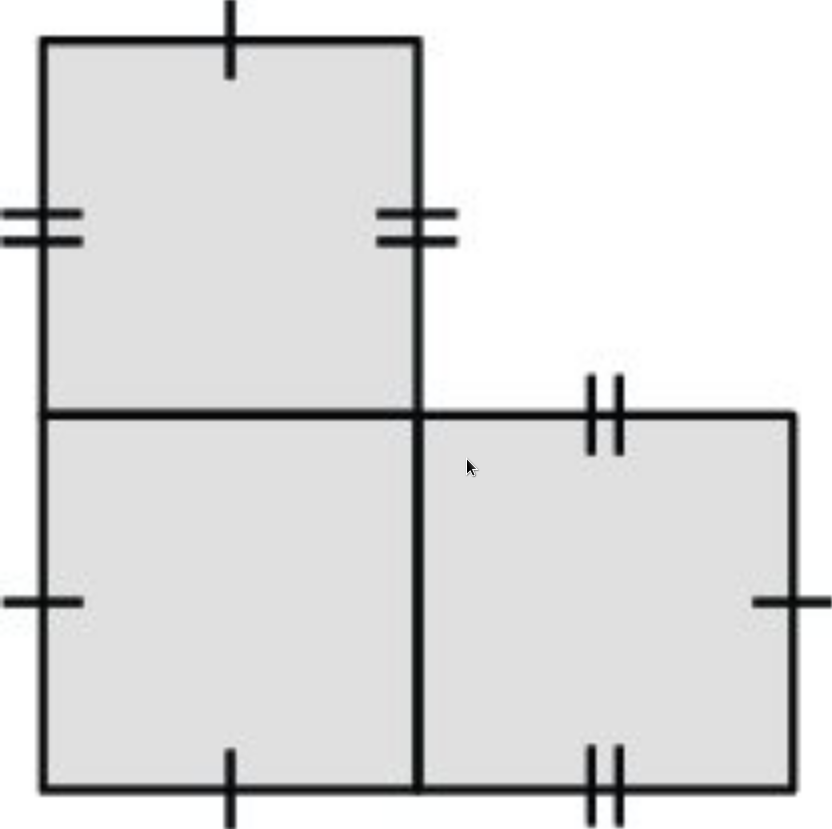
\includegraphics[width=\linewidth,height=0.5\textheight,keepaspectratio]{figures/cover.png}
  \end{center}
       \begin{minipage}{.35\linewidth}
    \begin{flushleft}
      \vspace{2em}
      {\fontsize{6pt}{2pt} \textit{Notes: These are notes live-tex'd
from a graduate course in Algebraic Curves taught by Pete Clark at the
University of Georgia in Fall 2020. As such, any errors or inaccuracies
are almost certainly my own. } } \\
    \end{flushleft}
    \end{minipage}
    \hfill
    \begin{minipage}{.65\linewidth}
    \end{minipage}
  }







\begin{document}

\date{}
\maketitle
\begin{flushleft}
\textbf{D. Zack Garza} \\
\textit{University of Georgia} \\
\textit{dzackgarza@gmail.com} \\
{\tiny \textit{Last updated:} 2020-10-28 }
\end{flushleft}


\newpage
\tableofcontents

\hypertarget{references-and-basics}{%
\section{References and Basics}\label{references-and-basics}}

\textbf{References:}

\begin{itemize}
\tightlist
\item
  Survey Paper: Anton Zorich,
  \href{https://arxiv.org/abs/math/0609392}{Flat Surfaces}
\item
  Alex Eskin, Andrei Okounkov,
  \href{https://arxiv.org/abs/math/0006171}{Asymptotics of numbers of
  branched coverings of a torus and volumes of moduli spaces of
  holomorphic differentials}
\item
  Alex Eskin, Howard Masur, Anton Zorich,
  \href{https://arxiv.org/abs/math/0202134}{Moduli Spaces of Abelian
  Differentials: The Principal Boundary, Counting Problems and the
  Siegel--Veech Constants}
\item
  Alex Eskin, Andrei Okounkov,
  \href{https://arxiv.org/abs/math/0505545}{Pillowcases and quasimodular
  forms}
\item
  Vincent Delecroix, Elise Goujard, Peter Zograf, Anton Zorich,
  \href{https://arxiv.org/abs/1903.10904}{Contribution of one-cylinder
  square-tiled surfaces to Masur-Veech volumes}

  \begin{itemize}
  \tightlist
  \item
    See Phil for appendix!
  \end{itemize}
\item
  Engel, \href{https://arxiv.org/abs/1706.06738}{Hurwitz Theory of
  Elliptic Orbifolds, I}
\item
  Engel, \href{https://arxiv.org/abs/1809.07434}{Hurwitz Theory of
  Elliptic Orbifolds, II}
\end{itemize}

\textbf{Definition:} A map \(\pi: \Sigma \to \Sigma'\) of Riemann
surfaces is said to be \emph{ramified} at a point \(p\in \Sigma'\) iff
in local charts \(\pi\) has the form \(z\mapsto z^n\) for some \(n>1\).

\begin{quote}
I.e. all points in a punctured neighborhood of \(\pi(p)\) have \(n\)
preimages.
\end{quote}

\textbf{Definition:} If \(\pi\) is ramified at \(p\), the number of
preimages \(n\) is referred to as \(e_p\), the \emph{ramification index
of \(p\)}.

\emph{Fact:} \(\vector{\beta}(\Sigma_g) = [1, 2g, 1, 0, \cdots]\) and
\(\chi(\Sigma) = 2-2g\).

\textbf{Theorem:} If \(\pi\) is an unramified covering map of degree
\(n\), then \(\chi(\Sigma') = n\chi(\Sigma)\).

\textbf{Theorem (Riemann-Hurwitz):} If \(\pi: \Sigma \to \Sigma'\) is a
ramified covering map of degree \(N\), then

\begin{align*}
\chi(\Sigma') = N \chi(\Sigma) - \sum (e_p - 1) \quad\text{ i.e. } 2 g(\Sigma') - 2=  N(2g(\Sigma) - 2)  + \sum (e_p - 1)
.\end{align*}

\emph{Another useful form:} Let \(r \in \Sigma'\) be the number of
ramification points, and \(b\) the number of branch points, i.e.~their
images in \(\Sigma\). Then

\begin{align*}
\chi(\Sigma') = N(\chi(\Sigma) - b) + r
.\end{align*}

\textbf{Holomorphic Forms:} A holomorphic \(p\dash\)form on \(X\) is a
section of \(\Lambda^p T\dual X\), the \(p\)th exterior power of the
holomorphic cotangent bundle of \(X\).

For \(n = \dim_\CC X\), the \(n\dash\)forms are an important special
case. Any such form \(w\) is given in local coordinates
\((z_1, \cdots, z_n)\) by

\begin{align*}
w = w(z_1, \cdots, z_n) dz_1 \wedge \cdots \wedge dz_n
\end{align*}

for some holomorphic function \(w: \CC^n \to ?\).

\textbf{Canonical Bundle:} Given a complex manifold \(M\), we can define
the tangent bundle \(\CC^n \to TM \to M\) and the cotangent bundle
\(\CC^n \to T\dual M \to M\), which we'll just denote \(T\dual M\). Then
the canonical bundle is the bundle \(\CC\to \Lambda^n T\dual M \to M?\),
denoted by \(\omega\), obtained by taking the \(n\)th exterior power.

It is a theorem that the fibers are in fact complex lines \(\CC^1\). For
vector bundles, this is referred to as the \emph{determinant bundle}. If
\(M\) is a smooth manifold, then \(\omega\) has a global section.

\begin{quote}
Note: a holomorphic \(n\dash\)form is exactly the same as a section of
the canonical bundle.
\end{quote}

Interesting aside: a Calabi-Yau is a manifold with a nowhere vanishing
holomorphic \(n\dash\)form, which implies that the canonical bundle
admits a map to a trivial line bundle that is an isomorphism, i.e.~the
canonical bundle is trivial.

\emph{Exercise:} For \(\Sigma_g\) a compact Riemann surface of genus
\(g\), the dimension of the space of holomorphic sections of the
canonical bundle, i.e.~the space of holomorphic differentials on
\(\Sigma_G\), is given by \(\dim H^0(X; \Omega) = g\) (the genus of the
surface). Proof: use Riemann-Roch.

Classification of elliptic orbifolds of dimension 2: Define
\((n_1, \cdots; m_1, \cdots)\) as the \emph{profile}, where \(n_i\) are
\emph{elliptic} points (locally look like quotient by \(\ZZ/n\ZZ\)), and
\(m_i\) are \emph{corner reflectors} (locally look like quotient by a
dihedral group):

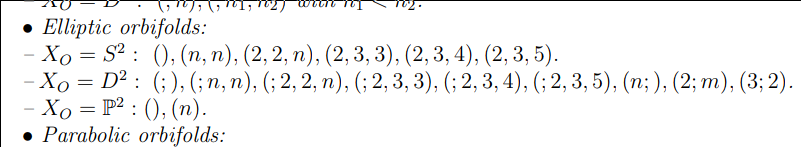
\includegraphics{figures/2020-01-29-20:44.png}\\

Conformal (or equivalently complex) structures on a genus \(g\) surface
form a moduli space \(\MM_g\) of dimension \(3g-3\) for \(g > 1\).

Let \(\alpha\) be any partition of \(2g-2\), and \(\mch(\alpha)\) the
moduli space of pairs \((\Sigma_g, \omega)\) where \(\Sigma_g\) is a
Riemann surface of genus \(g\) and \(\omega\) is a holomorphic 1-form
(Abelian differential) on \(M\) with the orders of its zeros given by
\(\alpha\). Letting \(\mch\) be the moduli space of all abelian
differentials on Riemann surfaces of genus \(g\) is stratified by
\(\mch(\alpha)\) as \(\alpha\) ranges over all partitions. For flat
tori, \(\mch = \GL_+(2, \RR)/\SL(2, \ZZ)\).

For \(\Sigma_g\) a Riemann surface, there is a formula (Gauss-Bonnet in
the flat metric) relating the degrees of the zeros of a holomorphic
1-form to the genus:

\begin{align*}
\sum d_j = 2g-2
.\end{align*}

\hypertarget{notes-on-paper}{%
\section{Notes on Paper}\label{notes-on-paper}}

\begin{quote}
Reference: \url{https://arxiv.org/abs/math/0609392}
\end{quote}

\hypertarget{section-1}{%
\subsection{Section 1}\label{section-1}}

Flat surfaces are characterized as surfaces with a flat metric and
(finitely many?) cone-like singularities. These surfaces appear to be
isomorphic to moduli spaces of holomorphic 1-forms. It is profitable to
study the orbit of the surface under the Teichmüller geodesic flow, as
well as a \(\GL_n\) action.

Some introductory surveys:

\begin{itemize}
\tightlist
\item
  A. Eskin {[}E{]},
\item
  G. Forni {[}For2{]},
\item
  P. Hubert and T. Schmidt {[}HuSdt5{]}
\item
  H. Masur {[}Ma7{]},
\item
  H. Masur and S. Tabachnikov {[}MaT{]}
\item
  J. Smillie {[}S{]}.
\end{itemize}

We usually associate

\begin{itemize}
\tightlist
\item
  Constant positive curvature = \(S^2\)
\item
  Constant zero curvature = \(S^1 \cross S^1 \definedas T^1 = \Sigma_1\)
\item
  Constant negative curvature = \(\Sigma_g\) for \(g\geq 2\), a surface
  of higher genus
\end{itemize}

\textbf{Proposition:} Any surface can be given a flat metric, possibly
introducing singular points.

\begin{quote}
Idea: Push all of the curvature into a cone point.
\end{quote}

\emph{Example:} The standard cube embedded in \(\RR^3\).

This is a flat surface with 8 cone points located at the vertices. Note
that the metric is non-degenerate on the edges, since any neighborhood
of a point on an edge is still homeomorphic to \(\RR^2\):

\begin{figure}
\centering
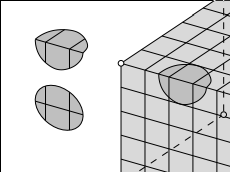
\includegraphics{figures/2020-01-11-23:54.png}
\caption{Image}
\end{figure}

Any neighborhood of a vertex is isometric to the vertex of the usual
notion of a cone. The cone angle can be measured by cutting a cone from
the base to the vertex, yielding a flat pattern that sits in \(\RR_2\),
and measuring the ``missing'' angle in the resulting circle:

\begin{figure}
\centering
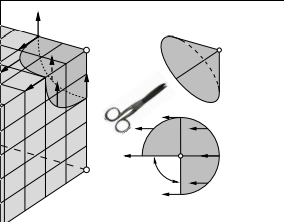
\includegraphics{figures/2020-01-12-00:00.png}
\caption{Image}
\end{figure}

This shows that the cone angle of the cube is \(3\pi/2\), which
coincides with the fact that there are 3 square (and thus 3 right
angles) adjacent to any cone point.

\textbf{Definition:} Geodesic (todo)

\textbf{Definition:} Ergodic (todo)

\begin{quote}
Here this means that a typical geodesic will visit any region in phase
space and time spent in a region is proportional to volume.
\end{quote}

\textbf{Definition:} Holonomy and Holonomy group (todo)

General (wildly open) problem:

\begin{itemize}
\tightlist
\item
  Describe the behavior of a generic geodesic on a surface
\item
  Prove that the geodesic flow is ergodic on a typical flat surface
\item
  Does almost every surface have a closed geodesic that does not pass
  through singular points?

  \begin{itemize}
  \tightlist
  \item
    If so, how many?
  \item
    Find the (asymptotic) number of such closed geodesics of length
    shorter than \(L\)
  \end{itemize}
\end{itemize}

This remains unsolved for \(S^2\) with 3 singularities (equivalent to a
certain billiards problem). It is not even known if any flat sphere
admits a single closed geodesic.

Flat surfaces have nontrivial holonomy, which makes them resemble
Riemannian manifolds more than flat tori.

If we take the surface and puncture the conical points, it is locally
isometric to the punctured Euclidean plane. This allows a notion of
parallel transport of tangent vectors.

Parallel transports along homotopically trivial loops are always the
identity; otherwise, for homotopically nontrivial loops this rotates the
vector by some angle. Parallel transport around a cone point rotates by
exactly the cone angle. Nontrivial holonomy forces geodesics to
self-intersect many times.

\begin{quote}
Exercise: parallel transport a vector around the cone point of a cube.
\end{quote}

The flat torus has trivial linear holonomy -- all geodesics either close
up, or never self-intersect and produce a dense winding path.

\textbf{Definition:} A translation surface is closed orientable surface
with a flat metric, a finite number of conical singularities, and
trivial linear holonomy.

Note that trivial linear holonomy implies that cone angles are all
integer multiples of \(2\pi\).

\begin{quote}
Convention: we assume all flat surfaces come with a distinguished
direction.
\end{quote}

Remark: Billiards gives rise to a flat surface with nontrivial linear
holonomy.

\textbf{Definition:} A half-translation surface is a surface with a flat
metric and holonomy group \(\ZZ/(2)\).

\begin{quote}
In this case, a vector \(\vector v\) may come back as \(-\vector v\)
after parallel transport.
\end{quote}

We'll often consider families of flat surface sharing the same genus and
number/type of conical singularities. These will correspond to strata of
moduli spaces of one-forms.

It will often be useful to let \(\SL(2, \RR)\) act on these families,
consider the orbits, and take its closure.

Central problem / conjecture: Taking the closure of an orbit under the
action of \(\GL^+(2, \RR)\) is a complex subvariety, so both the moduli
space of holomorphic one-forms and the moduli space of quadratic
differentials resemble homogeneous spaces under the action of a
unipotent group.

The there is a projection from these orbits (Teichmüller discs) to the
moduli space of complex structures (?), which will be denoted \(\MM_g\).
It is well-known that moduli spaces are not homogeneous spaces, but the
conjecture here is that they behave as if they were.

\hypertarget{section-2-motivations}{%
\subsection{Section 2: Motivations}\label{section-2-motivations}}

Open problems in rectangular billiards:

\begin{enumerate}
\def\labelenumi{\arabic{enumi}.}
\tightlist
\item
  Describe the behavior of a billiard trajectory in a generic triangle,
  and prove that the billiard flow is ergodic.
\item
  Does (almost) any table have at least one regular periodic trajectory?
  Is it preserved under deformations?
\item
  Asymptotically in length, how many periodic trajectories are there?
\item
  Does any obtuse triangle have a single periodic trajectory?
\end{enumerate}

\emph{Known example:} Acute triangles have at least 1, see Fagnano
trajectory

\emph{Fox-Kershner construction:} Yields a way to go from billiard
trajectories to geodesics on a flat surface. General idea: glue two
copies of the billiard table along the edge to get a flat sphere; then
paths lift to geodesics. Such surfaces are not ``very flat'', i.e.~they
have nontrivial linear holonomy.

\hypertarget{thursday-week-1}{%
\section{Thursday, Week 1}\label{thursday-week-1}}

\textbf{Motivation:} Gauss' Unicursal Problem. How many distinct curves
\(\alpha: [0, 1] \to \RR^2\) are there with no triple crossings?

Note that if we compactify the plane to the Riemann sphere (and possibly
take the curve to be piecewise linear) then we obtain a \emph{tiling} of
the sphere. We can also take a \emph{dual tiling} by taking the
barycenters of each polygon and connecting them by an edge iff their
corresponding polygons share an edge.

\textbf{Definition:} A \emph{translation surface} is the 2-dimensional
topological manifold obtained by taking any set of polygons in \(\RR^2\)
and gluing their edges by translations.

\emph{Example:} Any elliptic curve (topologically a torus) is a
translation surface.

We take equivalence up to cutting, pasting, and rearranging.

\textbf{Lemma:} Two elliptic curves (of genus 2) are isomorphic iff the
translation surfaces differ by a homothety, i.e.~a rotation and scaling.

\begin{quote}
Note: we will eventually see that the data of a translation surface is
equivalently a holomorphic 1-form.
\end{quote}

\textbf{Definition:} A \emph{half-translation surface} is a translation
surface where we now additionally allow gluing by rotations of \(\pi\)
radians.

\emph{Example:}

\begin{center}
\begin{tikzpicture}
        \node[fill=black, shape=circle]  (0) at (-3, 3) {};
        \node[fill=black, shape=circle]  (1) at (3, 3) {};
        \node[fill=black, shape=circle]  (2) at (-3, -3) {};
        \node[fill=black, shape=circle]  (3) at (3, -3) {};
        \node[fill=black, shape=circle]  (4) at (0, 3) {};
        \node[fill=black, shape=circle]  (5) at (0, -3) {};
        \draw (1.center) to node [auto] {$a$} (3.center);
        \draw (0.center) to node [left] {$a$} (2.center);
        \draw (0.center) to node [above] {$b$} (4.center);
        \draw (4.center) to node [above] {$b$} (1.center);
        \draw (2.center) to node [below] {$c$} (5.center);
        \draw (5.center) to node [below] {$c$} (3.center);
\end{tikzpicture}
\end{center}

\begin{quote}
Note that the gluing \(b\) now requires a rotation.
\end{quote}

By gluing edges with matching letters, we get a ``hot pocket'' surface:

\begin{center}
\begin{tikzpicture}[
    none/.style={text opacity=0,opacity=0,fill opacity=0},
    dashed/.style={text opacity=0,opacity=0,fill opacity=0}
]
        \node [style=none] (0) at (-3, 3) {};
        \node [style=none] (1) at (3, 3) {};
        \node [style=none] (2) at (-3, -4) {};
        \node [style=none] (3) at (3, -4) {};
        \node [style=none] (4) at (-3, 2) {};
        \node [style=none] (5) at (3, 2) {};
        \node [style=none] (6) at (-3, -0.5) {};
        \node [style=none] (7) at (3, -0.5) {};
        \node [style=none] (8) at (-3, -2.75) {};
        \node [style=none] (9) at (3, -2.75) {};
        \draw (0.center) to (2.center);
        \draw (2.center) to (3.center);
        \draw (3.center) to (1.center);
        \draw (0.center) to (1.center);
        \draw [bend right] (4.center) to (5.center);
        \draw[dotted] [bend left=15] (4.center) to (5.center);
        \draw [bend right] (6.center) to (7.center);
        \draw[dotted] [bend left=15] (6.center) to (7.center);
        \draw [bend right] (8.center) to (9.center);
        \draw[dotted] [bend left=15] (8.center) to (9.center);
\end{tikzpicture}
\end{center}

\textbf{Lemma:} Any game of \emph{rectangular billiards} yields a
half-translation surface.

Given any domain for rectangular billiards, we inflate it to a surface:

\begin{center}
\begin{tikzpicture}[
    none/.style={text opacity=0,opacity=0,fill opacity=0},
    dashed/.style={text opacity=0,opacity=0,fill opacity=0}
]
        \node [style=none] (0) at (-5, 6) {};
        \node [style=none] (2) at (0, 0) {};
        \node [style=none] (3) at (0, 4) {};
        \node [style=none] (4) at (3, 4) {};
        \node [style=none] (5) at (3, 2) {};
        \node [style=none] (6) at (6, 2) {};
        \node [style=none] (7) at (6, 6) {};
        \node [style=none] (8) at (-5, 0) {};
        \node [style=none] (9) at (-2.5, 6) {};
        \node [style=none] (10) at (-2.5, 0) {};
        \node [style=none] (11) at (1.5, 6) {};
        \node [style=none] (12) at (1.5, 4) {};
        \node [style=none] (13) at (4.5, 6) {};
        \node [style=none] (14) at (4.5, 2) {};
        \draw (0.center) to (8.center);
        \draw (8.center) to (2.center);
        \draw (2.center) to (3.center);
        \draw (3.center) to (4.center);
        \draw (4.center) to (5.center);
        \draw (5.center) to (6.center);
        \draw (6.center) to (7.center);
        \draw (0.center) to (7.center);
        \draw [bend right] (9.center) to (10.center);
        \draw[dotted] [bend left=15] (9.center) to (10.center);
        \draw [bend right=40] (11.center) to (12.center);
        \draw[dotted] [bend left=40, looseness=0.75] (11.center) to (12.center);
        \draw [bend right, looseness=0.75] (13.center) to (14.center);
        \draw[dotted] [bend left=15] (13.center) to (14.center);
\end{tikzpicture}
\end{center}

We can then cut along everything but the bottom edge to ``unwrap'' it
into a half-translation surface:

\begin{center}
\begin{tikzpicture}[
    none/.style={text opacity=0,opacity=0,fill opacity=0},
    dashed/.style={text opacity=0,opacity=0,fill opacity=0}
]
        \node [style=none] (0) at (-5, 6) {};
        \node [style=none] (2) at (0, 0) {};
        \node [style=none] (3) at (0, 4) {};
        \node [style=none] (4) at (3, 4) {};
        \node [style=none] (5) at (3, 2) {};
        \node [style=none] (6) at (6, 2) {};
        \node [style=none] (7) at (6, 6) {};
        \node [style=none] (8) at (-5, 0) {};
        \node [style=none] (9) at (-2.5, 6) {};
        \node [style=none] (10) at (-2.5, 0) {};
        \node [style=none] (11) at (1.5, 6) {};
        \node [style=none] (12) at (1.5, 4) {};
        \node [style=none] (13) at (4.5, 6) {};
        \node [style=none] (14) at (4.5, 2) {};
        \node [style=none] (17) at (-5, -6) {};
        \node [style=none] (18) at (6, -6) {};
        \node [style=none] (22) at (0, -4) {};
        \node [style=none] (23) at (3, -4) {};
        \node [style=none] (24) at (6, -2) {};
        \node [style=none] (29) at (3, -2) {};
        \draw (0.center) to node [auto] {$a$} (8.center);
        \draw (8.center) to (2.center);
        \draw (2.center) to node [auto] {$b$}  (3.center);
        \draw (3.center) to (4.center);
        \draw (4.center) to (5.center);
        \draw (5.center) to (6.center);
        \draw (6.center) to (7.center);
        \draw (0.center) to (7.center);
        \draw (8.center) to node [auto] {$a$} (17.center);
        \draw (17.center) to (18.center);
        \draw (2.center) to  node [auto] {$b$} (22.center);
        \draw (22.center) to (23.center);
        \draw (23.center) to (29.center);
        \draw (29.center) to (24.center);
        \draw (24.center) to (18.center);
\end{tikzpicture}
\end{center}

Some questions related to rectangular billiards:

\textbf{Question 1:} Given a random starting point and direction, what
proportion of the total region is traversed? Will the trajectory entire
a given region? How long does the billiard spend in any given region?

\textbf{Theorem:} The percentage of time spent in a given region is
equal to the proportion of its area to the total area.

\begin{quote}
This requires some ergodic theory.
\end{quote}

\textbf{Question 2:} If you shine a laser from a given spot, is the
entire region illuminated?

\textbf{Theorem:} No! There is a counterexample with 18 sides. Moreover,
no positive-area region can be avoided, but certain finite sets can.

\textbf{Definition:} A \emph{flat surface} is a generalization of
translation surfaces that now allows gluing by any isometry of
\(\RR^2\).

\emph{Example:} A cube in \(\RR^3\) is a flat surface, noting that the
planar gluing diagram for it now requires rotations of \(\pi/2\)
radians:

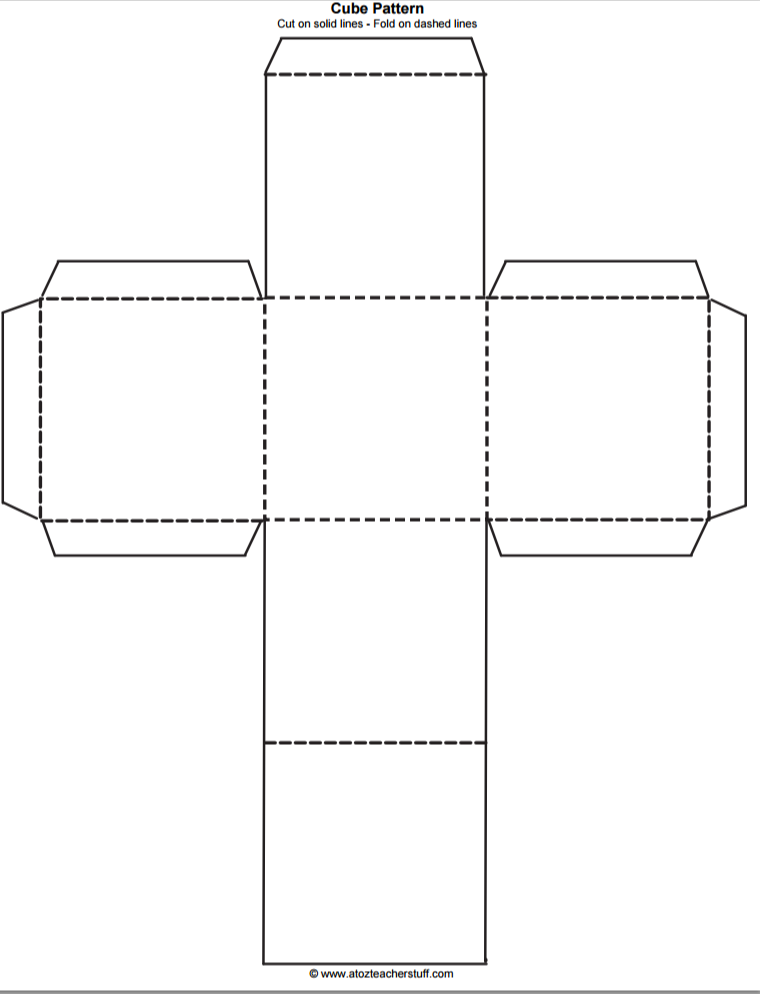
\includegraphics{figures/2020-01-11-22:16.png}\\

Note that we can form higher genus surfaces using polygon gluing:

\begin{center}
\begin{tikzpicture}[
    none/.style={fill=black,shape=circle,scale=0.5},
    dashed/.style={text opacity=0,opacity=0,fill opacity=0}
]
        \node[style=none] (0) at (-0.75, 2.5) {};
        \node [style=none] (1) at (0.75, 2.5) {};
        \node [style=none] (2) at (-1.75, 1.25) {};
        \node [style=none] (3) at (1.75, 1.25) {};
        \node [style=none] (4) at (-1.75, -0.25) {};
        \node [style=none] (5) at (1.75, -0.25) {};
        \node [style=none] (6) at (-0.75, -1.5) {};
        \node [style=none] (7) at (0.75, -1.5) {};
        \node [style=none] (8) at (-1.75, 1.25) {};
        \draw (0.center) to node [auto] {$d$}  (8.center);
        \draw (8.center) to node [auto] {$a$}  (4.center);
        \draw (4.center) to node [auto] {$b$}  (6.center);
        \draw (6.center) to node [auto] {$c$}  (7.center);
        \draw (7.center) to node [auto] {$d$}  (5.center);
        \draw (5.center) to node [auto] {$a$}  (3.center);
        \draw (3.center) to node [auto] {$b$}  (1.center);
        \draw (1.center) to node [auto] {$c$}  (0.center);
\end{tikzpicture}
\end{center}

\textbf{Exercise:} Check that there is only one vertex in this polygon.

In general, the vertices may have total angle greater than \(2\pi n\).
We refer to these as \emph{cone points}, and the total angle as the
\emph{cone angle}.

\textbf{Exercise:} Check that the cone angle in the above example is
\(6\pi\) by taking a loop around the cone point.

\begin{quote}
Note on a weird phenomenon: it seems difficult to find \(\ZZ^2\) or
\(\QQ^2\) points on the sloped edges of a regular polygon, based on
computer drawings.
\end{quote}

\emph{Remark:} This flat surface admits charts to \(\CC\) with the
following transition functions. Let \(P\) denote the single cone point.

Then there is a 3-fold cover give by the following space, thought of as
a singular helical

\begin{center}
\begin{tikzpicture}[
    none/.style={fill=black,shape=circle,scale=0.5},
    dashed/.style={text opacity=0,opacity=0,fill opacity=0}
]
    \draw (0, 0) circle (3cm);
    \node [style=none, label=P] (0) at (0, 0) {};
    \node [style=none] (1) at (3, 0) {};
    \draw (0.center) to node [above] {$C$} node [below] {$A$} (1.center);

    \draw (0, -7) circle (3cm);
    \node [style=none, label=P] (0) at (0, -7) {};
    \node [style=none] (1) at (3, -7) {};
    \draw (0.center) to node [above] {$A$} node [below] {$B$} (1.center);

    \draw (0, -14) circle (3cm);
    \node [style=none, label=P] (0) at (0, -14) {};
    \node [style=none] (1) at (3, -14) {};
    \draw (0.center) to node [above] {$B$} node [below] {$C$} (1.center);

\end{tikzpicture}
\end{center}

which maps onto the unit disc in \(\CC\):

\begin{center}
\begin{tikzpicture}[
    none/.style={fill=black,shape=circle,scale=0.5},
    dashed/.style={text opacity=0,opacity=0,fill opacity=0}
]
    \draw (0, 0) circle (3cm);

    \node [style=none, label=P] (P) at (0, 0) {};
    \node [style=none] (u1) at  ({1*360/3}: 3cm){};
    \node [style=none] (u2) at  ({2*360/3}: 3cm){};
    \node [style=none] (u3) at  ({3*360/3}: 3cm){};

    \draw (P) to (u1);
    \draw (P) to (u2);
    \draw (P) to (u3);

    \node [label=1] (u1) at  ({1*360/6}: 1.5cm){};  
    \node [label=2] (u1) at  ({3*360/6}: 1.5cm){};
    \node [label=3] (u1) at  ({5*360/6}: 1.5cm){};

\end{tikzpicture}
\end{center}

The covering map from the former to the latter is given by
\(z\mapsto z^{\frac 1 3}\), which coincides with the fact that the cone
angle at \(P\) is \(3(2\pi) = 6\pi\).

One can also imagine this space in \(\RR^3\) with a projection onto the
plane: \pgfplotsset{compat=1.16,width=10cm,height=14cm}

\begin{center}
\begin{tikzpicture}
\begin{axis}[trig format plots=rad,
        view={-40}{6*pi},
        colormap={adopted}{
            rgb255(0cm)=(219,0,70);
        rgb255(1cm)=(55,70,170);
            rgb255(2cm)=(219,0,70)
        },
        z buffer=sort,
        zmin=0]
\addplot3 [surf,domain=0.001:4,domain y=-pi/2:6*pi-pi/2,samples=25,samples y=40]
({x*cos(y)},{x*sin(y)},{ln(x)+y});
\end{axis}
\end{tikzpicture}
\end{center}

Here the helicoid goes through three full twists, where the top and
bottom pieces are identified.

\textbf{Proposition:} In a neighborhood of a cone point \(P\) with cone
angle \(2\pi n\), the map \(z\mapsto z^{\frac 1 n}\) will be a local
chart for any \(z\) in a neighborhood of \(P\).

This gives the resulting surface the structure of a \emph{Riemann
surface}, i.e.~a surface admitting charts to \(\CC\) with holomorphic
transition functions.

Let \(X\) be a Riemann surface, we can look at the \emph{canonical
bundle} over \(X\) with sections that are compatible collections of
\(f_u(z_u) ~dz_u\) for each chart \(z_u\), and for each such chart a
holomorphic function \(f_u(z_u)\) on \(z_u(U)\) where on overlaps

\begin{align*}
f_u(z_u) ~dz_u &= f_v(z_v) ~dz_v \\
&= f_v(z_v \circ z_u) z_v'(z_u) ~dz_u
.\end{align*}

\textbf{Updated Definition:} A \emph{translation surface} is a Riemann
surface with a section of its canonical bundle.

\emph{Example:} \(C/\Lambda\) for \(\Lambda\) any rank-2 lattice:

\begin{figure}
\centering
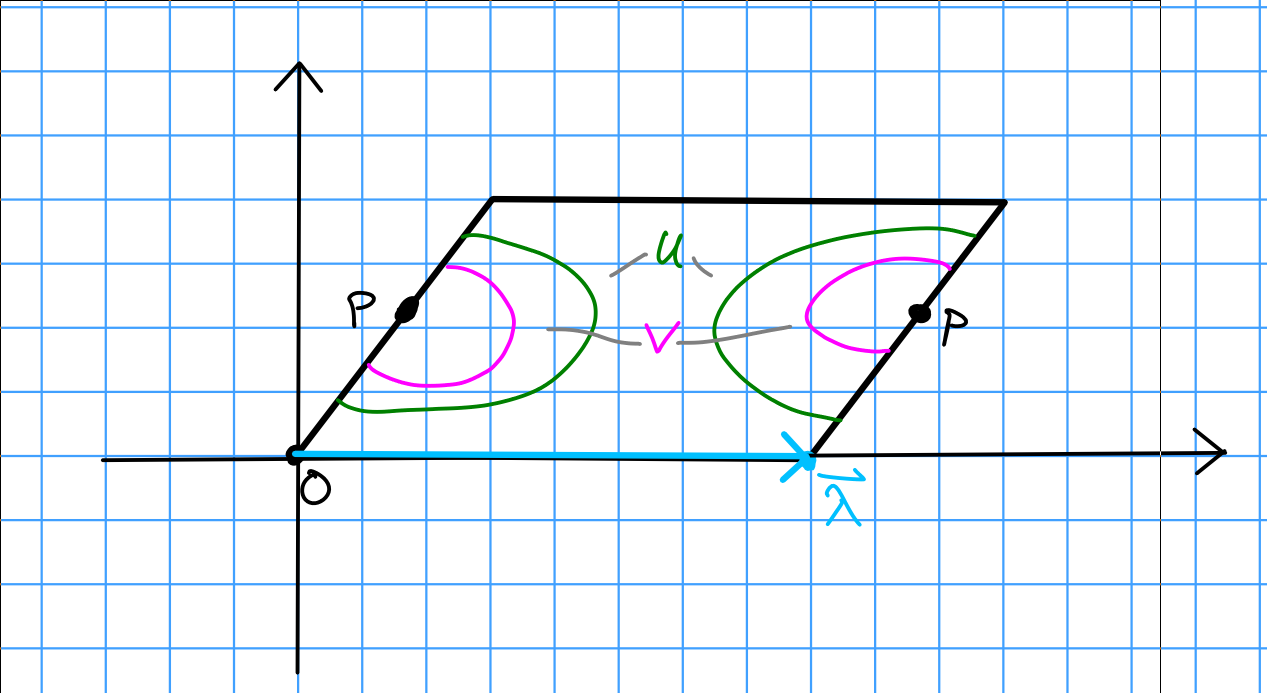
\includegraphics{figures/2020-01-11-23:35.png}
\caption{Image}
\end{figure}

\begin{quote}
Note that the translation here is given by \(\vector \lambda\).
\end{quote}

\textbf{Definition:} A holomorphic 1-form is a section of the canonical
bundle.

\emph{Example:} For the above surface, we have
\(z_v = z_u + \vector \lambda\) and thus \(dz_u = dz_v\) is
nonvanishing.

Note that \(dz\) is a holomorphic 1-form on the complement of the
vertex/vertices of the polygon.

\textbf{Proposition:} \(dz\) extends holomorphically to charts
containing cone points with cone angle \(2\pi n\) and has a zero of
order \(n-1\) at such cone points.

\emph{Example:} For the chart \(z=w^3\) where \(w\) is the local
coordinate, we have \(dz = 3w^2\), yielding a zero of order 2.

\hypertarget{thursday-january-16th}{%
\section{Thursday January 16th}\label{thursday-january-16th}}

\hypertarget{correspondence}{%
\subsection{Correspondence}\label{correspondence}}

\textbf{Recall:} Start with a translation surface with cone points with
angles \(2\pi n i\). This yields a Riemann surface \(\Sigma\) and a
holomorphic \(1\dash\)form \(\omega\) with zeros of order \(n_i -1\).

Given a square fundamental domain, there is an order 4 automorphism
given by rotating 90 degrees. In charts, this is multiplication by \(i\)
and possibly a translation, which is a holomorphic map
\(f: \Sigma \selfmap\). We then have \(f^*(dz) = d(f(z)) = idz\), so
\(dz\) is an eigenvector for \(f^*\).

An elliptic curve can be specified by \(y^2 = f_4(x)\) for a degree 4
polynomial, so we can obtain it as a double branched cover of \(S^2\).
(i.e.~glue along the slits joining pairs of roots)

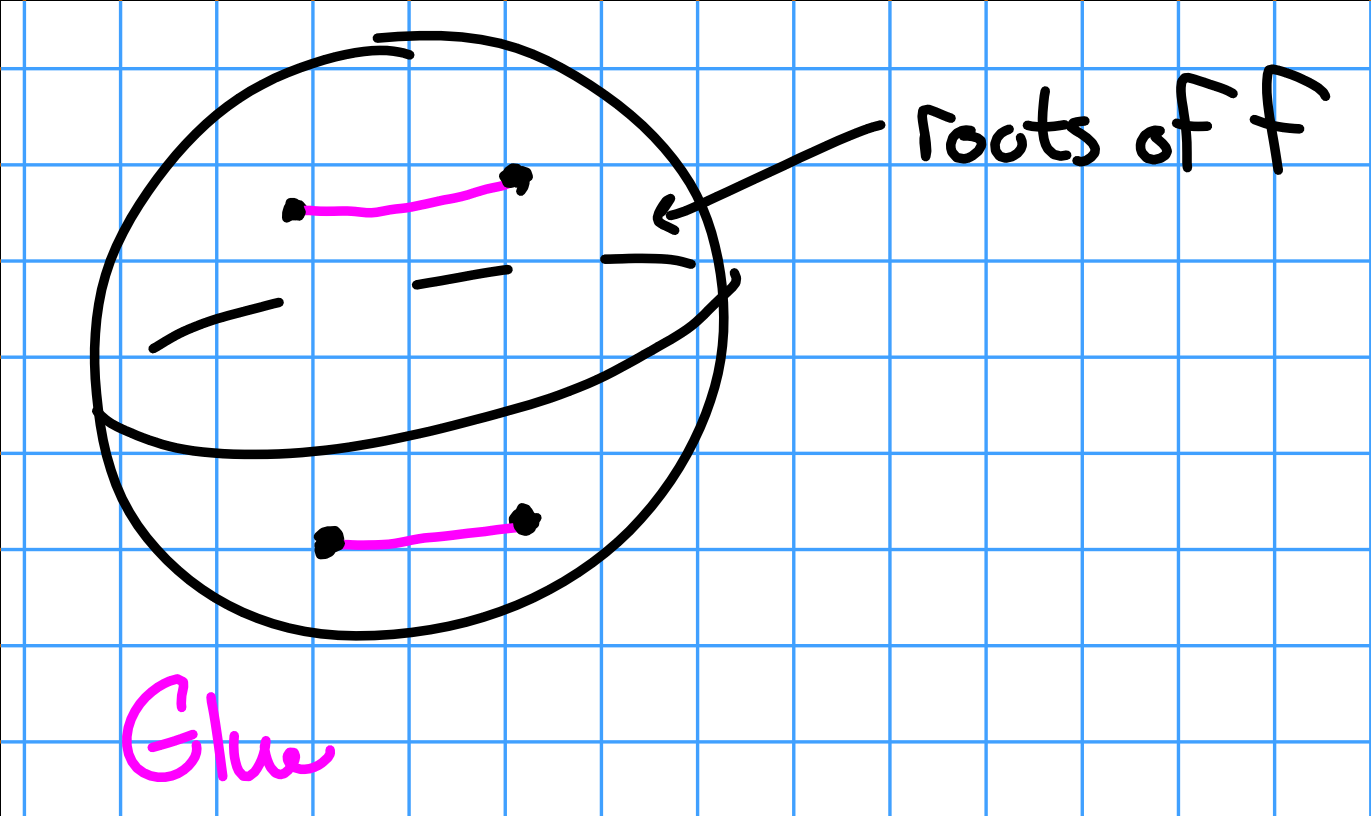
\includegraphics{figures/2020-01-22-21:56.png}\\

Take \(E : y^2 = x^4 - 1\), this is the only elliptic curve with an
order 4 automorphism. In coordinates, this is generated by
\((x, y) \mapsto (-ix ,y)\). So \(\omega = c \frac{dx}{y}\),
i.e.~\(dx/y\) up to scaling, and \(f^*(dx/y) = i \frac{dx}{y}\). What is
the constant \(c\)?

Take closed cycles on \(E\) given by \(\alpha, \beta\) (see diagram),
then by FTC \(\int_\alpha \omega = z \mid_0^1 = 1\). Negation is 4 fixed
points on the elliptic curve, the 2-torsion points.

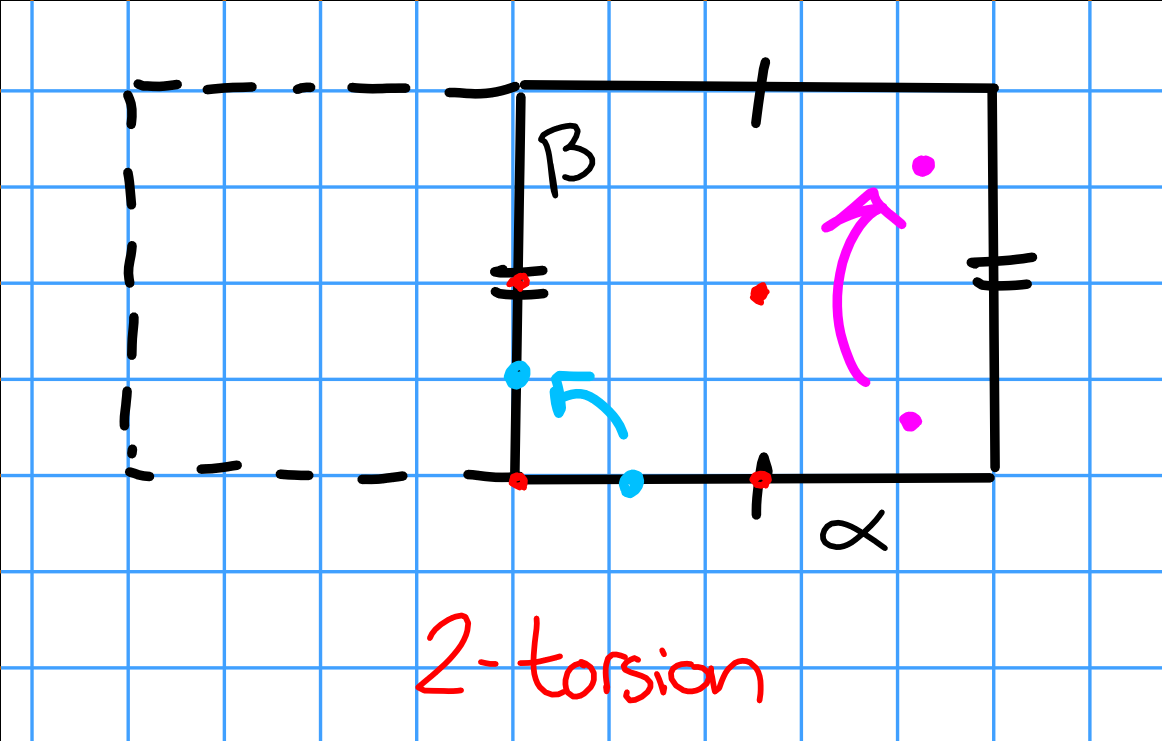
\includegraphics{figures/2020-01-22-21:55.png}\\

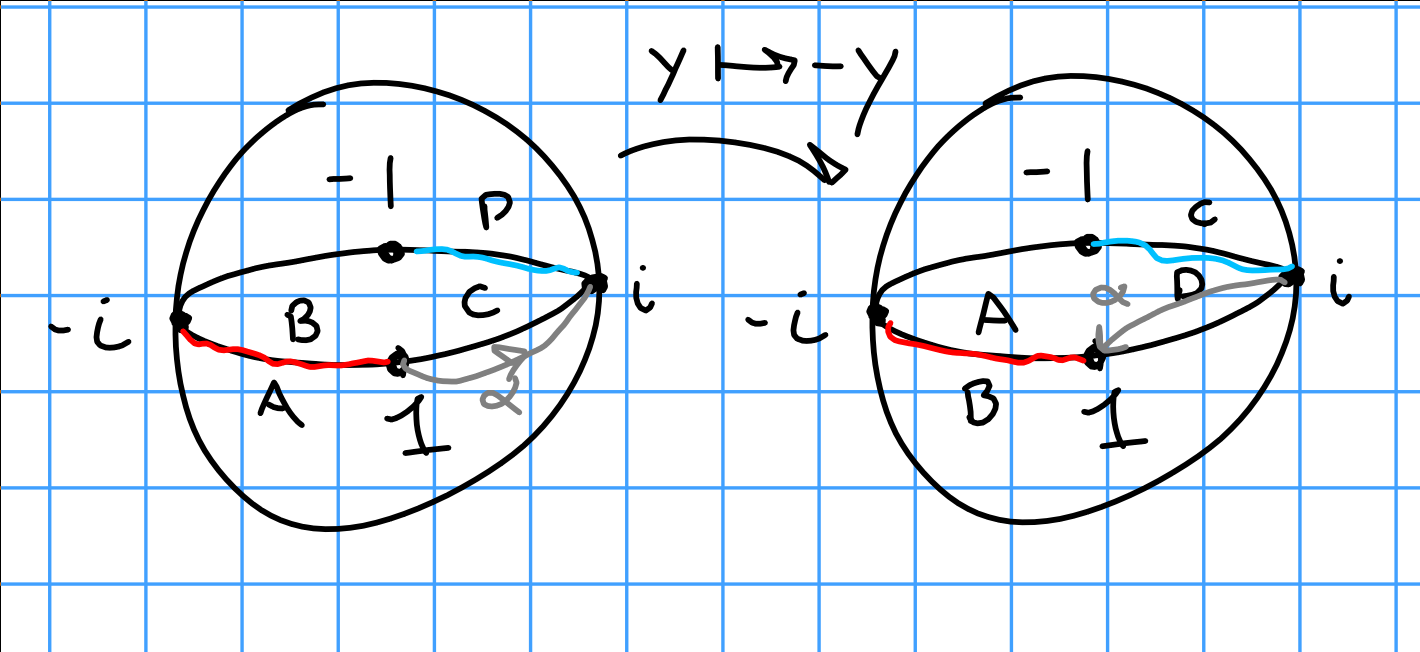
\includegraphics{figures/2020-01-22-21:57.png}\\

We can then compute

\begin{align*}
I = \int_\alpha  \frac{dx}{y} = \int_1^2 \frac{dx}{\sqrt{x^4 - 1}} 
.\end{align*}

and since \(2c I = 1\), this uniquely determines \(c\).

\begin{quote}
Note that this can be numerically evaluated, but this is an elliptic
integral with (possibly) no elementary antiderivative.
\end{quote}

Consider the decagon with sides identified. We get a complex structure
\((\Sigma, \omega)\) with cone angles \(4\pi\) and \(dz\) has 2 zeros of
order 1 (namely the two cone points).

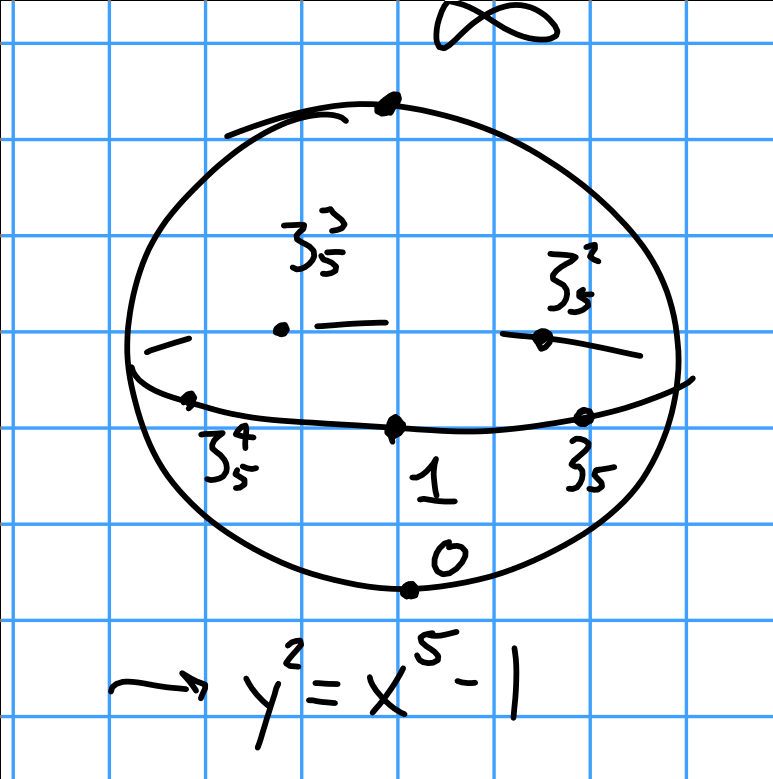
\includegraphics{figures/2020-01-22-21:58.png}\\

What is the genus? The degree of the canonical bundle is
\begin{align*}
g(\Sigma) = \deg K_\Sigma = 2g - 2 = \sum_{p\in \Sigma}\ord_p \omega
\end{align*} and thus \(g = 2\).

\textbf{Fact:} Every genus 2 curve is a double branched cover of
\(\PP^1\) branched over 6 points.

\begin{quote}
Use Riemann-Roch.
\end{quote}

Consider automorphisms that preserve the decagon. Rotation by \(\pi/10\)
swaps the two cone points, to take rotation by \(-2\pi/5\) (inserting
the negative to account for pullbacks). Then
\(f^* \omega = \zeta_5 \omega\), where again we just write locally
\(z \mapsvia{f} \zeta_5\inv + c \implies f^* dz = \zeta_5 dz\).

Consider points of order \(5\) on \(\PP^1\), we can take \(\zeta_5^k\)
and \(\infty\).

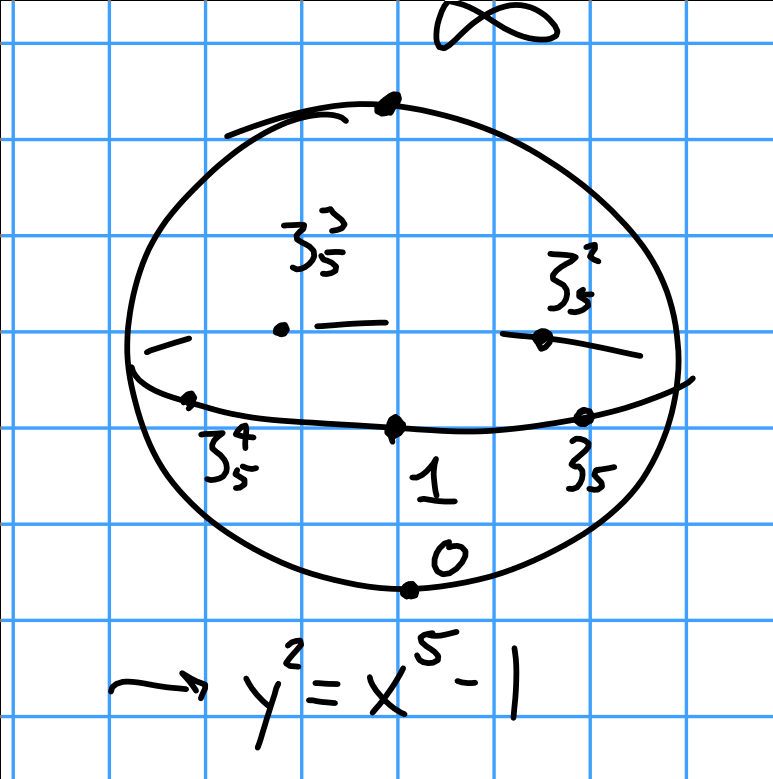
\includegraphics{figures/2020-01-22-21:58.png}\\

This corresponds to the curves \(y^2 = x^5 - 1\), with an automorphism
\((x, y) \mapsto (\zeta_5 x, y)\). This is the only genus 2 curve with
an order 5 automorphism.

\textbf{Fact:} The space of sections of the canonical
\(H^0(K_{\mathcal E}) = \CC^g\).

We can write a basis for the space of 1-forms: \(\frac{dx}{y}\) and
\((1-x) \frac{dx}{y}\). Alternatively, \(\omega = (a+bx) \frac{dx}{y}\)
where \(a, b \in \CC\). What are the zeros of \(\omega\)?
\(V(\omega) = V(a + bx)\) where if \(b=0\) it's \(\infty\). Because this
has to preserve the order 5 symmetric and map cone points to themselves,
this forces \(\omega = bx \frac{dx}{y}\), which has exactly two zeros:
\((x, y) = (0, \pm i)\).

We can also consider the doubled pentagon, which has only one point.
This has an automorphism given by rotating each pentagon by \(1/5\), it
has cone angle \(6\pi\), and \(\omega\) has a double zero at the cone
point. Since there is only \emph{one} genus 2 curve with order 5
automorphisms, this yields the previous Riemann surface but a distinct
translation surface and a distinct form.

We can write \(\alpha = a \frac{dx}{y}\).

\textbf{Proposition:} One Riemann surface has many translation
structures, and the space of such structures is the space of 1-forms.

\emph{Proof:} Pick a chart \(w: U \to \CC\) avoiding the zeros of
\(\omega\). Then \(\omega = f(z) ~dz\) in this chart, and we want to
compose with a biholomorphism \(x\) to obtain a new chart \(z\) such
that \(\omega = dz\) in this chart. We can solve \(dz = e = f(w) ~dw\)
and \(\frac{dz}{dw} = f(w)\) and by integrating we get
\(z(w) = \int_{p_0}^w f(w_0) dw_0\). In this chart, \(\omega = dz\), and
we can correct near zeros by finding charts such that
\(\omega = z^n dz\) where \(n\) is the order of the zero.

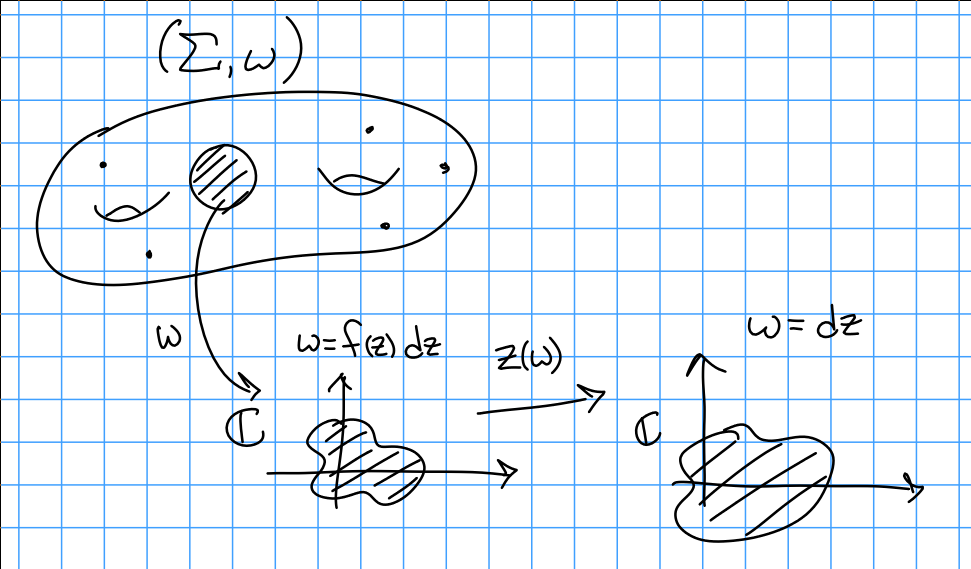
\includegraphics{figures/2020-01-22-21:59.png}\\

What does this buy us? We get a translation structure by considering
transitions, and \(\omega = dz_1 = dz_2 \implies z_1 = z_2 + c\), which
is exactly a translation structure. Thus every \((\Sigma, \omega)\) has
a translation structure for which \(\omega = dz\) in local polygonal
charts.

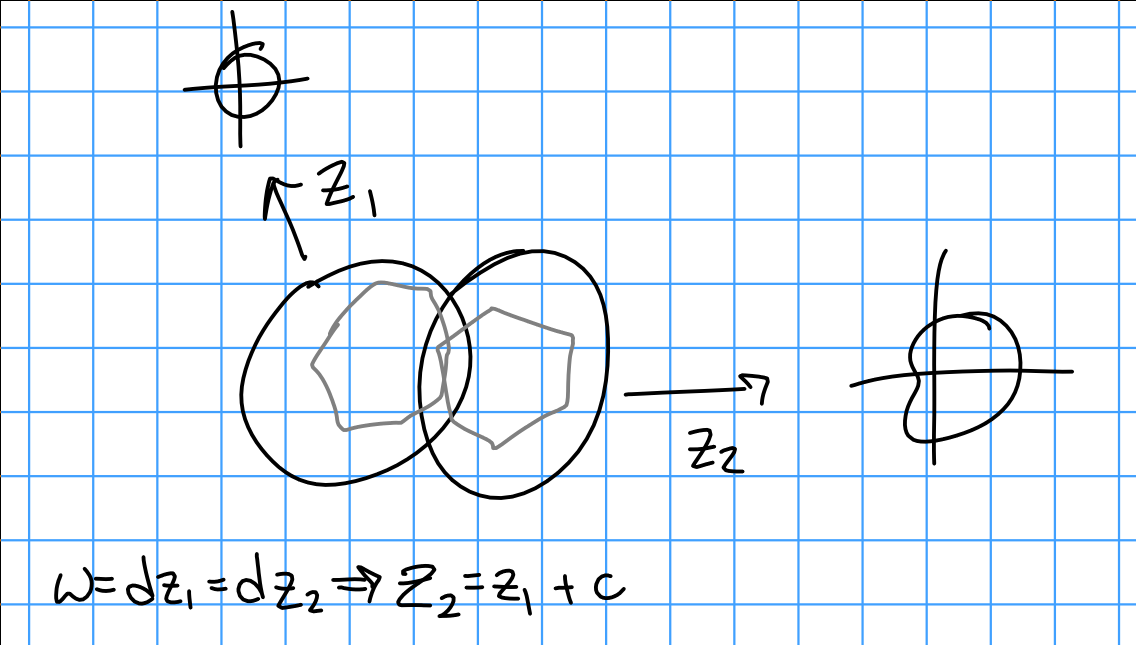
\includegraphics{figures/2020-01-22-22:00.png}\\

\textbf{Theorem:} There is a bijection

\begin{align*}
\correspond{\text{Translation surfaces with cone angles $2\pi n i$ }} \iff
\correspond{\text{$(\Sigma, \omega)$ a Riemann surface with holomorphic}\\ \text{1-forms with zeros of order $n_i - 1$}}
.\end{align*}

What do half-translations correspond to? Note that \(dz \mapsto -dz\),
so we don't get a well-defined holomorphic 1-form.

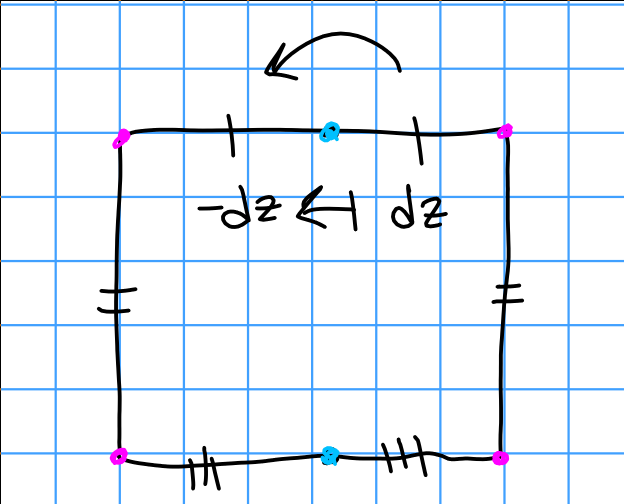
\includegraphics{figures/2020-01-22-22:01.png}\\

The fix? \((dz)^2\) is some well-defined object. What is it?

The set \(\theset{f(z) (dz)^2 = g(w)(dw)^2}\) corresponds with line
bundles with transition functions given by \((dz/dw)^2\).

Thus the correspondence is

\begin{align*}
\correspond{\text{Half translation surfaces with cone angle $\pi n_i$}}
\iff
\correspond{\text{Riemann surfaces with $q$ a section of $K_\Sigma^{\tensor 2}$ }}
.\end{align*}

I.e., these correspond with sections of the second tensor power of the
canonical bundle of \(\Sigma\).

A defining property of \(q = (dz)^2\) for half-translation charts \(z\):
we can measure the order of the zero by going to charts, finding a chart
to \(\CC\) (see image) e.g.~\(w = z^{2/3}\), and then defining
\begin{align*}
\omega = dz = d(w^{3/2}) = 3/2 w^{1/2} dw
\end{align*}

Then \(q = w^2 = (dz)^2\) is well-defined and equal to
\(\frac{9}{4} w (dw)^2\) in the local chart \(w\).

In this case, we get points that are \emph{poles} of order 1 for the
quadratic differential (sections of \(K^{\tensor 2})\).

\begin{quote}
Note: 1-forms are referred to as ``abelian differentials'' in the
literature.
\end{quote}

We know that \(K_{\PP^1} = \mathcal O(-2)\) and
\(K_{\PP^1}^{\tensor 2} = \mathcal O(-4)\).

\hypertarget{moduli-spaces}{%
\subsection{Moduli Spaces}\label{moduli-spaces}}

\textbf{Definition:}
\(\mathcal{H}(k_1, \cdots, k_n) = \theset{ \Sigma \text{ with abelian differential} \div \omega = \sum k p_i}\)
where the \(k_i\) record the orders of zeros of \(\omega\).

\begin{quote}
Second condition on divisor records zeros.
\end{quote}

Similarly, define
\(Q(k_1, \cdots, k_n) = \theset{\cdots \suchthat \text{quadratic differential}}\)
where now \(k_i \geq -1, \neq 0\).

These moduli spaces are called \emph{strata of abelian/quadratic
differentials}.

Consider \(M_g\), the moduli space of genus \(g\) surfaces. There is a
vector bundle (the Hodge bundle) over \(M_g\) where the fiber over
\([c]\) is \(H^0(K_C)\) with strata given by \(Q\).

This is a bundle of rank \(g\), and by Riemann-Roch, ? \(3g-3\) and is
the (co?)tangent bundle of something.

There is an \(\SL(2, \RR)\) action on any stratum. How to define -- use
isomorphism with translation structures (see image) by just applying any
such form \(\gamma\) to the entire plane and gluing polygons in the same
way. This gives a non-holomorphic action on any stratum.

\begin{quote}
Next time: to special case of square tiled surfaces.
\end{quote}

\hypertarget{thursday-january-23rd}{%
\section{Thursday January 23rd}\label{thursday-january-23rd}}

\hypertarget{counting-square-tiled-surfaces}{%
\subsection{Counting Square Tiled
Surfaces}\label{counting-square-tiled-surfaces}}

Square tiled surfaces in \(\mch(k)\) with \(d\) squares correspond to
degree \(d\) branched covers of the identification square, branched over
the origin, with profile (?).

To count square-tiled surfaces: label squares, look at inverse images of
\(\ast\) by \(\theset{1 ,\cdots, d}\). Consider the monodromy
representation \(\rho: \pi_1( \TT \setminus \theset{0}, \ast ) \to S_d\)
where \(\sigma = \rho(\alpha) = (1)(23)\) and
\(\tau = \rho(\beta) = (12)(3)\). We compute ramification orders by
considering the commutators \([\alpha, \beta]\). Then
\(\rho([\alpha, \beta] )\) has cycle type
\((1, 1, \cdots 1, 1+k, \cdots, 1+ k_n)\). Note that \([(23), (12)]\) is
a 3 cycle.

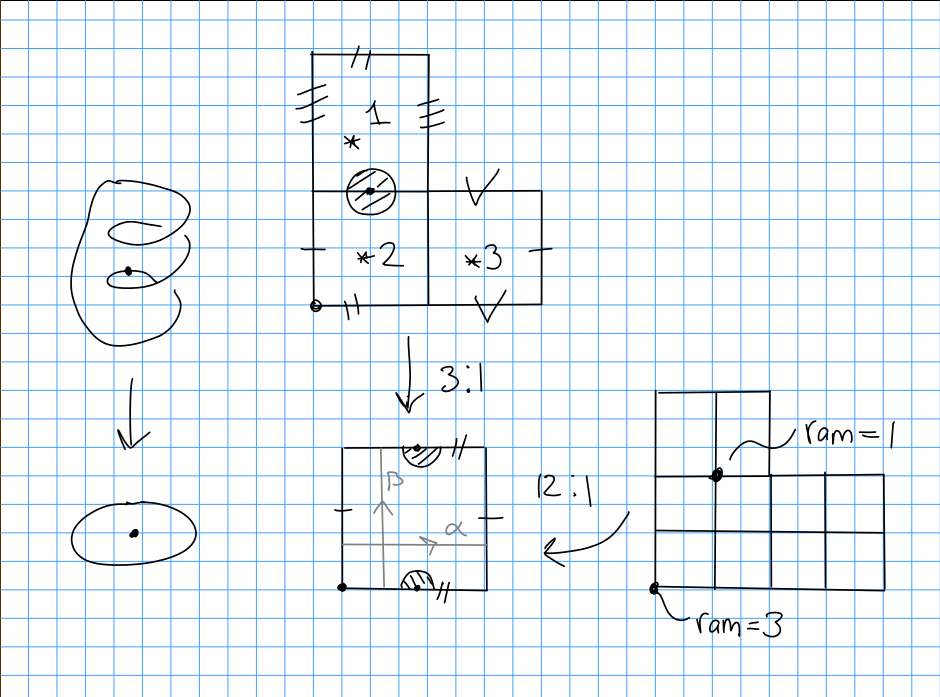
\includegraphics{figures/2020-01-23-14:32.png}\\

\textbf{Conclusion:} The number of square-tiled surfaces in \(\mch(k)\)
with \(d\) squares is exactly
\begin{align*}
\frac{1}{d!} \abs{\theset{\sigma, \tau \in S_d \suchthat [\sigma, \tau] \in C_{1, \cdots, 1, 1+k, \cdots, 1+ k_n}}}
.\end{align*}

Note that the division is due to the artificial labeling of squares.

\textbf{Main theorem from ``Branched Covers of Torus'' Paper:} The
generating function
\begin{align*}
f_\kappa(q)\definedas \sum_{d\geq 1} \#\theset{\text{Square tiled, $d$ squares in $\mch(k)$}} q^d
\end{align*} is a \textbf{modular form}.

Follows from taking \(q = e^{2\pi i \tau}\) which is holomorphic on
\(\HH\) the upper half-plane, satisfying a transformation rule with
respect to \(\tau \mapsto -1/\tau\), which is a finite-dimensional
space.

\begin{quote}
Actual: quasimodular mixed form.
\end{quote}

The weights are bounded by \(\abs \kappa + \ell(\kappa)\).

Concretely, \(f_\kappa \in \QQ[E_2, E_4, E_8]\) where
\(E_k(q) = \text{const} + \sum_{d \geq 1} \sigma_{k-1}(d) q^d\), where
\(\sigma_{k-1}(d) = \sum_{e\mid d} e^{k-1}\). This is the ring of
quasimodular forms.

\begin{itemize}
\tightlist
\item
  \(1\) is weight 0,
\item
  \(E_2\) is weight 2,
\item
  \(E_2^2, E_4\) are weight 4,
\item
  \(E_2^3, E_2 E_4, E_6\) are weight 6, etc
\end{itemize}

\emph{Example:} Take \(\kappa = \theset{2} \iff \mch(2)\), then
\(\abs \kappa + \ell(\kappa) = 3\) and
\(f_{\theset z}(q) = c_1 + c_2 E_2(q)\). In this case
\([q^1] = [q^2] = 0\).

Note that surfaces in \(\mch(2)\) have 1 vertex of cone angle \(6\pi\)
and all others of angle \(2\pi\), corresponding to an abelian
differential with a single zero of order 2.

A special type of square-tiled surfaces: 1 cylinder surfaces, where
\(\rho(\alpha)\) is a full length cycle.

This is in \(\mch(3, 1)\), and corresponding surface
\((\Sigma, \omega)\), which is a holomorphic 1-form with a triple zero
and a single zero. By Riemann-Hurwitz,
\(2g-2 = \deg \omega = 3+1 \implies g = 3\).

\begin{quote}
Note: the genus here difficult to compute otherwise!
\end{quote}

\textbf{Main Result of 1-Cylinder Surface Paper:} 1-cylinder surfaces
have roughly a \(1/d\) proportion in all square tiled surfaces, where
\(d = \dim \mch(\kappa)\).

Recall that we can get a square tiled surface from any unicursal curve:

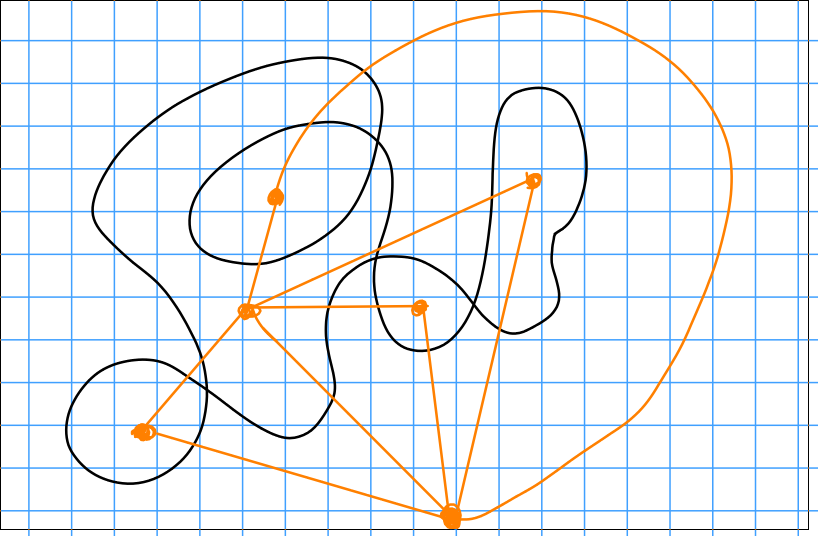
\includegraphics{figures/2020-01-23-14:41.png}\\

Note that these aren't always translation surfaces:

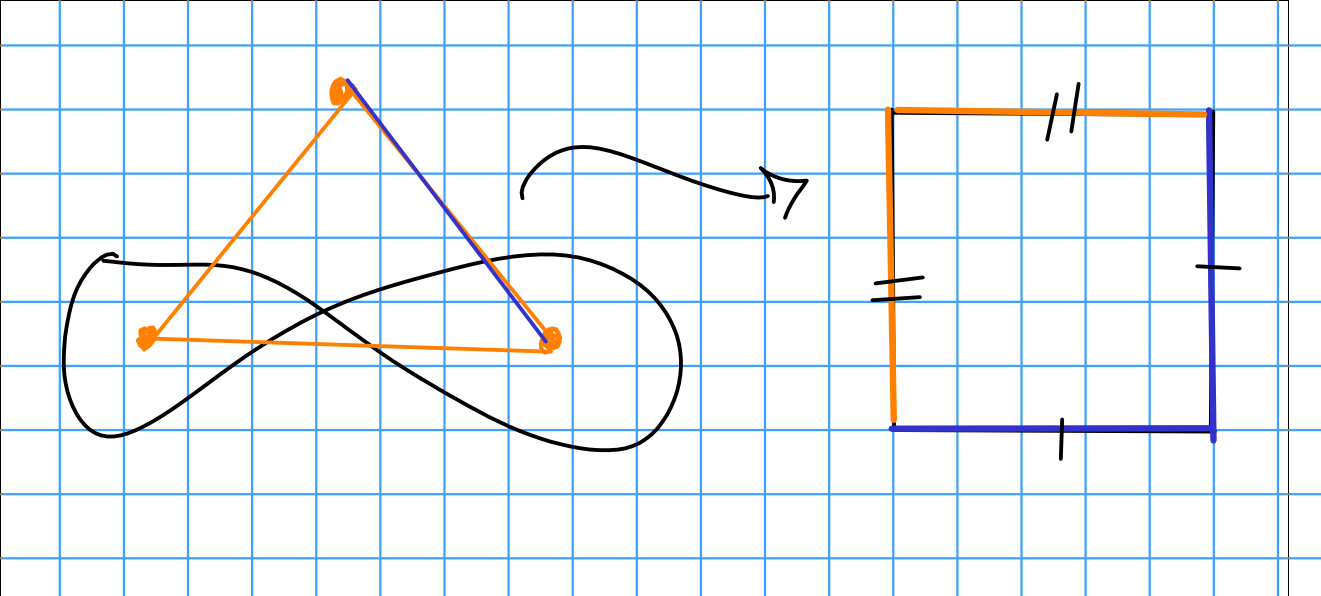
\includegraphics{figures/2020-01-23-14:43.png}\\

This has transition maps that looks like \(z \mapsto i^k z + z_0 = w\)
and thus \(dz = i^k dw\), so \(dz^k\) is the well-defined object here.

Recall

\begin{itemize}
\tightlist
\item
  \((\Sigma, dz) \iff\) translation surfaces
\item
  \((\Sigma, (dz)^2) \iff \frac 1 2 \dash\)translation surfaces
\item
  \((\Sigma, (dz)^4) \iff \frac 1 4\dash\)translation surfaces

  \begin{itemize}
  \tightlist
  \item
    I.e. a Riemann surface with a section of \(K_\eps^{\tensor 4}\).
  \end{itemize}
\end{itemize}

Can consider a \emph{tricursal} curve instead (a curve that requires
lifting the pen 3 times). Taking the dual complex yields a cube.

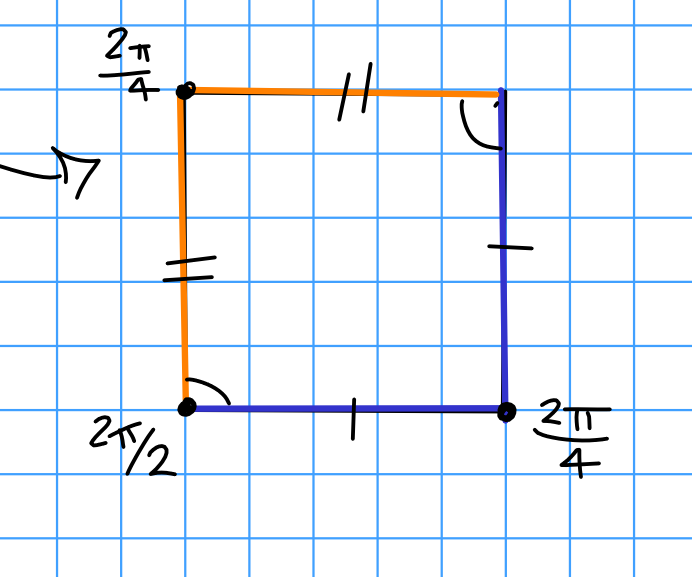
\includegraphics{figures/2020-01-23-14:52.png}\\

This has charts \(w = z^{4/3}\) and thus \((dz)^4 = w\inv (dw)^4\). Let
\(\mch(\kappa)\) be the quartic differentials with
\(dv \omega = \sigma \kappa_i p_i\). Then the cube is in
\(\mch_4(-1, \cdots -1)\) with \(8\) copies of \(-1\).

This gives cone angles \(n \frac{2\pi}{4}\) and the order of the
zero/pole is \(n-4\).

This example is in \(\mch_4(-3, -3, -2)\).

\textbf{Proposition:} The generating functions for square-tiled surfaces
\(\mch_4(\kappa)\) is now a quasimodular form for \(\Gamma_1(4)\).

\hypertarget{open-questions}{%
\subsection{Open Questions}\label{open-questions}}

\textbf{Question (can find numerical evidence?):} How can we count these
in terms of the symmetric group? Analogous result to proportion result
earlier? Can try to lift square example, but admits no map from a torus
-- instead, quotient square by \(\ZZ/4\ZZ\) and take fundamental domain.
What kind of branching do these covers have?

Every center of a square is branched of order 4. Every center of an edge
is branched of order 2. The ramification order of a vertex is its
valence, divided by the number of squares meeting at that vertex. The
degree of the covering map is \(4n\) where \(n\) is the number of
squares.

Identify the fundamental domain with \(\PP^1\), We get a monodromy
representation:

\begin{align*}
\rho: \pi_1(\PP^1 \setminus(0, 1,\infty), \ast) \to S_{4d} \\
\gamma_0 \mapsto \rho(\gamma_0)
.\end{align*}

Note that \(\gamma_0 \gamma_1 \gamma_\infty = 1\).

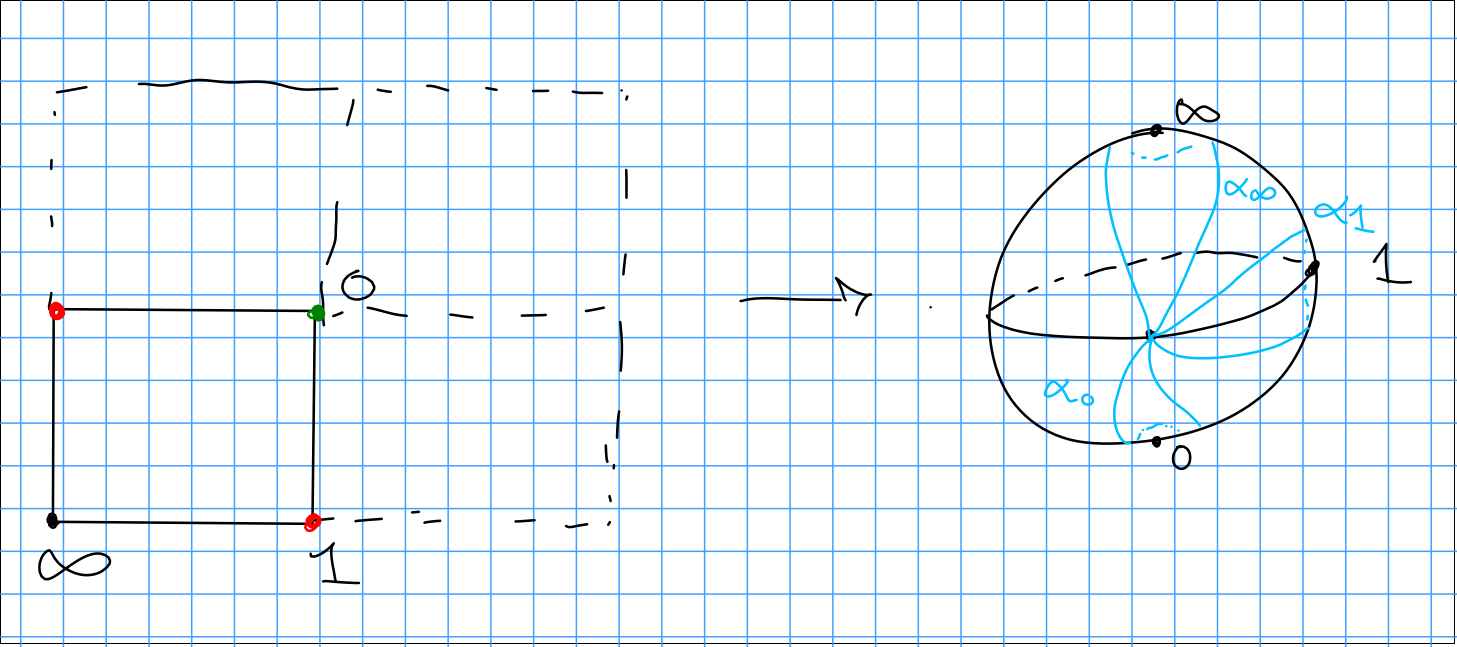
\includegraphics{figures/2020-01-23-15:13.png}\\

It then follows that this has cycle type \((4, \cdots ,4)\).

So the number of square tiled surfaces in \(\mch_4(\kappa)\) is given by

\begin{align*}
\frac{1}{(4d)!} = \# \theset{ (\sigma_0, \sigma_1, \sigma_\infty) \suchthat \sigma_0 \in C_{4, \cdots, 4} (d), \sigma_1 \in C_{2, \cdots ,2} (2d), \sigma_{\infty} \in C_{4, \cdots ,4, 4+k, \cdots, 4 + k_n}, \sigma_0 \sigma_1 \sigma_\infty = 1}
.\end{align*}

Would be nice to figure out what the proportionality constant here is.

\hypertarget{bens-talk-eskins-ramified-coverings-of-a-torus}{%
\section{Ben's Talk: Eskin's Ramified Coverings of a
Torus}\label{bens-talk-eskins-ramified-coverings-of-a-torus}}

Today: Section 2. Main theorem: a certain generating function is
quasimodular.

Consider a torus \(T\) with marked points
\(Z = \theset{z_1, \cdots z_s}\) with a map \(\sigma: \Sigma \to T\)
which is \emph{unramified} outside of \(Z\).

\begin{figure}
\centering
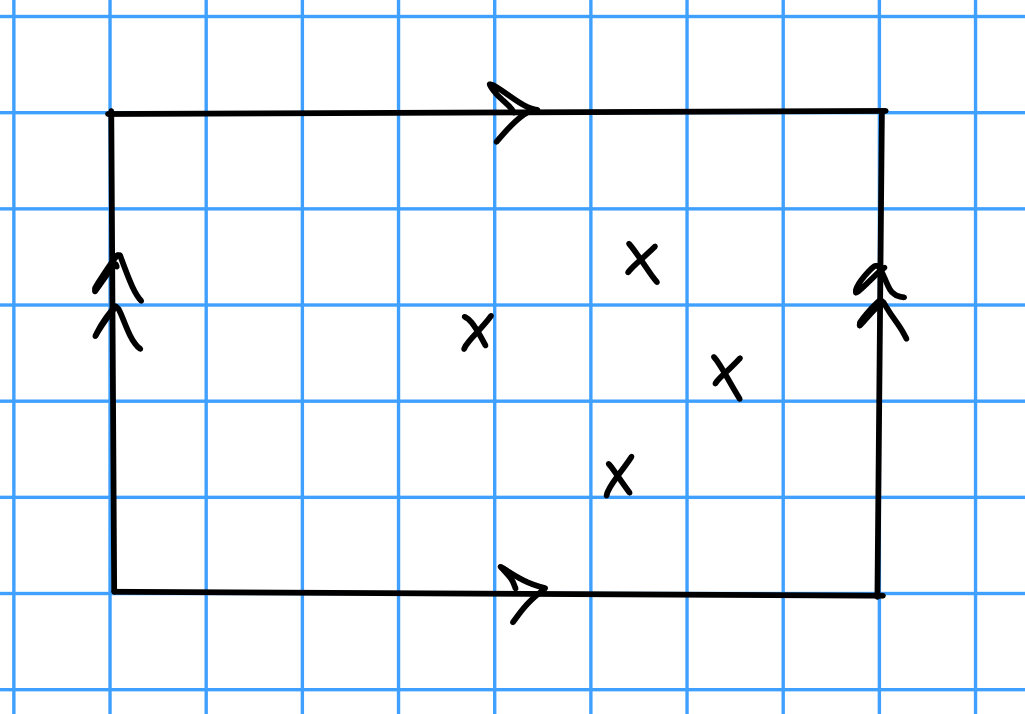
\includegraphics{figures/2020-01-30-14:04.png}
\caption{Image}
\end{figure}

Then \(\sigma\) is determined by the representation
\(\pi_1(T\setminus Z, \ast) \to \Aut(\sigma\inv(\ast)) \cong S_d\) if
\(\sigma\) is a degree \(d\) cover. There is a correspondence

\begin{align*}
\correspond{\text{d-fold covers ramified over } \theset{z_i}} 
\iff
\hom(\pi_1(T\setminus Z, \ast), S_d)
.\end{align*}

Fix \(C_1, \cdots, C_s\) conjugacy classes in \(S_d\), and let
\(H_d(C_1, \cdots, C_s)\) be the homomorphisms sending small loops
around \(z_i\) to \(C_i\).

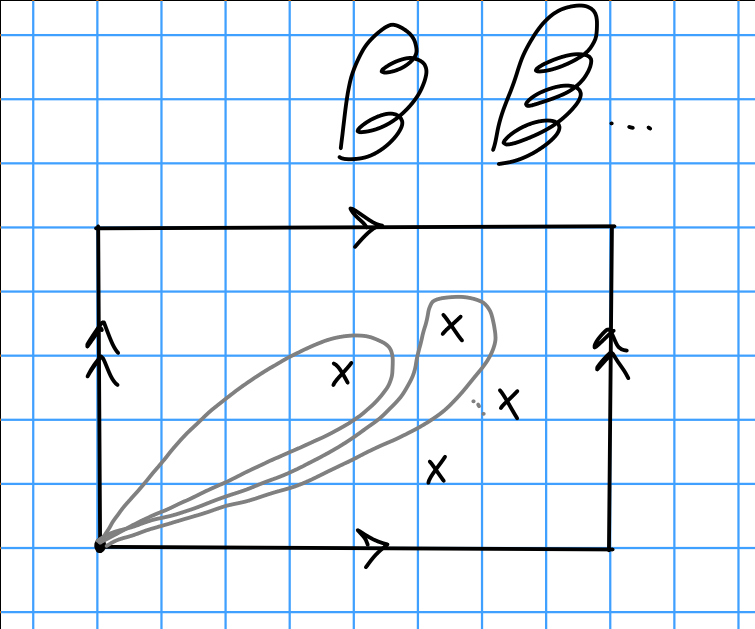
\includegraphics{figures/2020-01-30-14:09.png}\\

Then cycle types correspond to branching orders over points.

One way to count d-fold covers is to look at the weights of
\(\Aut(\sigma)\). We define

\begin{align*}
\mathrm{Cov}_d (C_1, \cdots, C_s) = \sum_{\sigma \in H_d(C_i) / S(d)} \frac{1}{\abs{\Aut(\sigma)}} = \frac{\abs{H^d(C_1, \cdots, C_2)}}{d!}
.\end{align*}

This just yields a number, so we can define a generating function:

\begin{align*}
\mathrm{Cov}(C_1, \cdots, C_s) = \sum_{d=0}^\infty q^d \mathrm{Cov}_d(C_1, \cdots, C_s)
.\end{align*}

\textbf{Important note:} To make sense of \(C_i\) in all \(S^d\), write
\(C_i = (m_{i1}, \cdots , m_{ik})\) and set \(\mathrm{Cov}_d(C_i) = 0\)
iff \(i_k < d\), and otherwise pad with 1s to get
\(C_i \definedas (m_{i1}, \cdots, m_{ik}, 1, 1, \cdots)\).

\emph{Remark:} The generating function counts all (possibly)
disconnected covers. Example: \(\mathrm{Cov}(\wait)\) counts all
unramified covers, and \(\phi(C_1, \cdots C_s)\) counts connected
covers. These generating functions will end up being quasimodular.

\textbf{Definition}: Set
\(H_d^1(C_1, \cdots, C_S) \subset H_d(C_1, \cdots, C_S)\) be the degree
\(d\) coverings \emph{without} unramified components.

\textbf{Definition}: Set
\(\mathrm{Cov}'(C_1, \cdots, C_S)= \sum q^d \frac{\abs{H_d^1(C_1, \cdots, C_s)}}{d!}\).

This yields the generating function for number of coverings without
unramified components.

\textbf{Lemma}:
\(\mathrm{Cov}' (C_1, \cdots, C_S) = \mathrm{Cov}(C_1, \cdots, C_S) / \mathrm{Cov}()\).

\emph{Sketch of proof:} Look at coefficients in the expansion

\begin{align*}
\abs{H_d(C_1, \cdots, C_S)} = \sum_{k=0}^d {d\choose k} \abs{H_k(C_1, \cdots , C_S)} \cdot \abs{H_{d-k}()}
.\end{align*}

Recall that \(\mathrm{Cov}_d(C_1, \cdots C_S)\) correspond to \(S_d\)
representations of \(\pi_1(T\setminus Z)\), and we can get a
presentation
\begin{align*}\pi_1(T\setminus Z) = \generators{\sigma, \gamma, g_i \suchthat [\omega,\gamma] \prod g_i = e}
.\end{align*}

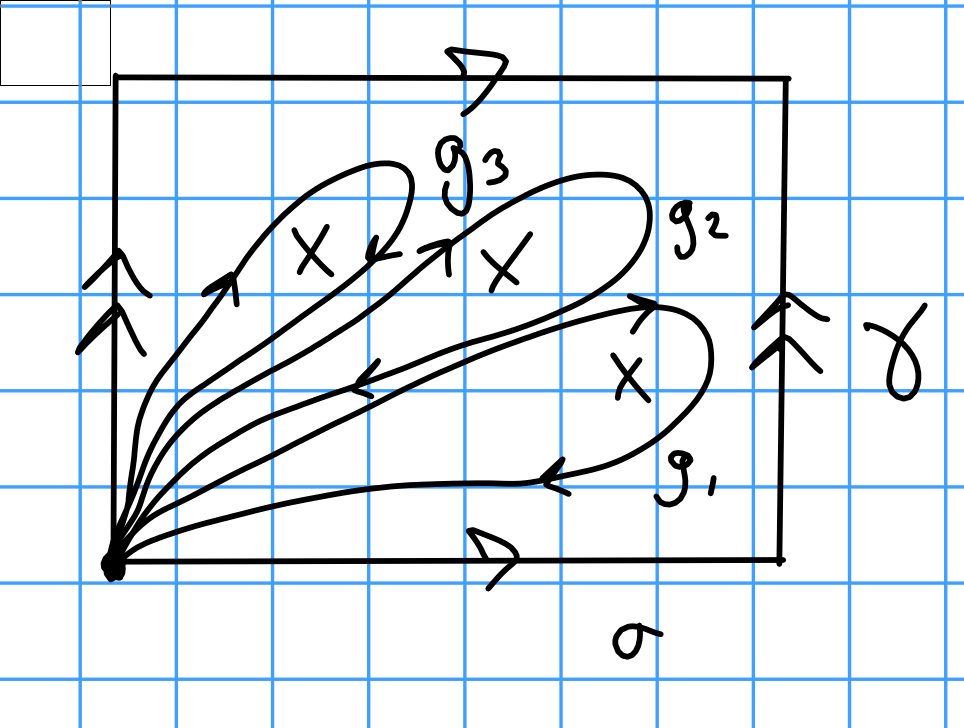
\includegraphics{figures/2020-01-30-14:33.png}\\

\begin{quote}
This just comes from doing one full loop around the outside square,
which should be equivalent (up to orientation) to going around all 3
punctures.
\end{quote}

\textbf{Definition:} Conjugacy classes corresponds to partitions of
\(d\).

\textbf{Definition:} For \(C\) a conjugacy class correspond to a
partition \(\lambda'\) in \(S_d\). For any partition \(\lambda\), let
\(f_C(\lambda) = \# C \chi^\lambda(C) / \dim \lambda\), where
\(\chi^\lambda\) is the irreducible representation associated to
\(\lambda\) (note that this is a rescaling of a row of the character
table, since irreducible reps happen to correspond to conjugacy classes
for \(S_d\)). This is a class function, so \(\chi^\lambda(C)\) is its
value on any \(c\in C\), and
\(\dim \lambda \definedas \chi^\lambda(1)\).

\textbf{Proposition:}
\(\mathrm{Cov}_d(C_1, \cdots, C_S) - \sum_{\abs \lambda = d} \prod_{i=1}^S f_{C_i}(\lambda)\).

\emph{Proof:} Let
\(\prod C_i = \prod \sum_{a_j\in C_i} a_j \in Z(\CC[S_d])\). Why?
Commutating elements reindexes the sum here.

We also have \(\sum_{g, h} [g, h] \prod C_i \in Z(\CC([S_d]))\), since
\([g ,h]^k = [g^k, h^k]\), which again just reindexes the sum.

We'll pull out a factor of \(\frac 1 {d!} [\id]\), and consider what the
coefficient of \([\id]\) is in the group algebra.

Thus
\(\frac{1}{d!} [\id] = \frac{1}{(d!)^2} \tr_{\text{reg}}\qty{ \sum [g, h] \prod C_i }\),
where we consider the regular representation: multiplying by elements of
\(g\) is a fixed-point free action, so these are traceless (no terms on
the diagonal) whereas the trace of the identity is exactly the dimension
of the regular representation, which is \(d!\) (?).

Thus we define
\(\tr_{\text{reg}}(\wait) = \sum_{\lambda} (\dim \lambda) \tr_\lambda(\wait)\).

Note that \(\rho: S_d \to \GL(V)\) extends to
\(\rho: \CC[S_d] \to \endo(V)\), and thus by Schur's Lemma, the image of
the center will commute with every endomorphism.

We get a formula:

\begin{align*}
\frac{[\id]}{d!} 
&= \frac{1}{(d!)^2} \sum_{\abs \lambda = d} \dim \lambda \tr_{\lambda}(\sum [g, h] \prod_i C_i) \\
&= \sum_{\abs \lambda = d} \frac{(\dim \lambda)^2}{(\abs \lambda !)^2} W(\lambda) \tr_\lambda(\prod C_i)
.\end{align*}

where \(W(\lambda)\) is a scalar \(\sum [g, h]\) by the above
observation.

Recall that \(f_c(\lambda) = \# C \frac{\chi^\lambda(C)}{\dim \lambda}\)
and thus

\begin{align*}
\frac{[\id]}{d!} = \sum_{\abs \lambda = d} \qty{\frac{\dim \lambda}{\abs \lambda}}^2 W(\lambda) \prod f_{C_i}(\lambda)
.\end{align*}

\textbf{Fact:}
\(W(\lambda) = \qty{\frac{\abs \lambda !}{\dim \lambda}}^2\).

\hypertarget{quasimodularity}{%
\subsection{Quasimodularity}\label{quasimodularity}}

\textbf{Fact:} The functions \(f_C(\lambda)\) are polynomial functions
in the following way:

\textbf{Definition:} Let \(\Lambda^*(n)\) be the algebra of ``shifted
symmetric functions'', i.e.~symmetric functions in the
\(\lambda_i - i\).

\begin{quote}
Subtlety: it's necessary to order to partition in weakly decreasing
order of the numbers occurring! Example:
\(p(\lambda) = (\lambda_1 - 1)(\lambda_2 - 2)\), but swapping
\(\lambda_1 \iff \lambda_2\) results in
\(((\lambda_2 - 2) + 1)((\lambda_1 - 1) - 1)\) is no longer symmetric in
\(\lambda_i - i\).
\end{quote}

Then define \(\Lambda^* = \lim_{\from} \Lambda^*(n)\).

\begin{quote}
Schur-Weyl duality: bijects representations of \(\GL_n\) and \(S_n\).
\end{quote}

Then \(f_c \in \Lambda^*\) and the degree of \(f_C\) is exactly the
number of non-fixed points of any permutation from \(C\).

From the paper,

\begin{align*}
\mathrm{Cov}(C_1, \cdots, C_S) &= \sum_\lambda q^{\abs \lambda} \prod_i f_{C_i}(\lambda) \\
\mathrm{Cov}() &= \sum a^{\abs \lambda} = \qty{ \prod_{n\geq 1} 1-q^n }\inv = (q)_\infty\inv
.\end{align*}

\begin{quote}
Note: the partition functions appears!
\end{quote}

For any \(F\in \Lambda^*\), we set
\(\generators{F}_q = (q)_\infty \sum_\lambda q^{\abs \lambda} F(\lambda)\)
and
\begin{align*}
\generators{F_1 \mid F_2 \mid \cdots \mid F_S}_q = \sum_{\alpha\in \pi_S} (-1)^{\phi(\alpha) - 1} (\phi(\alpha) - 1)! \prod_{k=1}^{\phi(\alpha)} \generators{\prod_{i\in\alpha_j} F_i}_q
.\end{align*}

\begin{quote}
This comes from Möbius inversion, and is a form of inclusion-exclusion.
\end{quote}

\textbf{Proposition:}
\(\mathrm{Cov}'(C_1, \cdots, C_S) = \generators{f_{C_1} \cdots f_{C_S}}_q\)
and
\(\phi(C_1, \cdots, C_S) = \generators{f_{C_1} \mid \cdots \mid f_{C_S}}_q\).

\textbf{Theorem:} For all \(F\in \Lambda^*\), \(\generators{F}_q\) is a
quasimodular form, i.e in \(\CC[E_2, E_4, E_6]\) where
\(E_i(q) = \const + \sum \sigma+{i-1} (n) q^n\).

\newpage

\newpage
\section{Indices}
\listoftodos[List of Todos]

% Hook into amsthm environments to list them.
\renewcommand{\listtheoremname}{Definitions}
\listoftheorems[ignoreall,show={definition}, numwidth=3.5em]

\renewcommand{\listtheoremname}{Theorems}
\listoftheorems[ignoreall,show={theorem,proposition}, numwidth=3.5em]

\renewcommand{\listtheoremname}{Exercises}
\listoftheorems[ignoreall,show={exercise}, numwidth=3.5em]

\listoffigures


\printbibliography[title=Bibliography]


\end{document}
